% Grundlagen & verwnadte Arbeiten

\chapter{Aktueller Stand der Technik}
\label{grundlagen}
%-------------------------------------------------------------
\section{AR in der Medizin}												 %
%-------------------------------------------------------------
\label{relatedAR}
Der Nutzen, den AR-Anwendungen in der Medizin darstellen wurde bereits von zahlreichen Arbeiten belegt, von denen einige im Folgenden vorgestellt werden. 
Obwohl die Einsatzgebiete dabei vielfältig sind, sind die Mehrzahl der Arbeiten für einen operativen Kontext konzipiert. Ein weiterer Schwerpunkt ist die Visualisierung von dreidimensionalen MRT-Daten in AR bzw. VR. %Die Einsatzbereiche sind dabei vielfältig. Beispielsweise stellen \cite{Voinea16} eine AR-Anwendung vor die den Lernprozess im Bereich der Biomechanik unterstützt.

\subsection{Bildgestütze medizinische Eingriffe}

Ein großer Anwendungsbereich ist der Einsatz von AR in der Ausführung und Vorbereitung von Operationen. Bei einem chirurgischen Eingriff kann für den Patienten ein hohes Risiko, eventuell sogar Lebensgefahr bestehen. Deshalb ist es wichtig, dass der operierende Arzt sich bestmöglich auf seine Aufgabe vorbereiten kann, wobei AR-Anwendungen ihn unterstützen können.
Die Kerneigenschaft von AR ist die Fähigkeit der Technologie, die Umgebung des Nutzers mit zusätzlichen Informationen anzureichern. Im Rahmen einer Operation bedeutet das Daten und Bildmaterial zum Fall des Patienten anzuzeigen. Um dem Arzt bei der Orientierung während des Eingriffs zu unterstützen ist es sinnvoll ihm anatomische Bilder zur Verfügung zu stellen, die er vorher bereits studiert hat. Diese stammen meist aus zuvor erzeugten MRT-Daten, die unter Umständen weiterverarbeitet wurden. Durch AR können diese in Echtzeit an der realen Positionen angezeigt werden. 
Die folgenden Arbeiten haben sich mit der Umsetzung dieses Konzeptes beschäftigt.


% Andere Hardware
Während ein Patient sich in einem MRT-Scanner befindet, können die MRT-Bilder direkt an den Arzt weitergeleitet werden. Dieser kann diese zur besseren Orientierung bei z.B. Injektionen nutzen. Offene MRT-Systeme\footnote{Erläuterung offener/geschlossener MRT-Systeme in Abschnitt \ref{mrt}.} ermöglichen dabei eine Abbildung der betroffenen Organe während des Eingriffs. Die Bildqualität ist allerdings deutlich schlechter als bei geschlossenen Systemen. Bei einem geschlossenen System hat der Arzt dagegen während des Scans keinen Zugang zum Patienten. Um einen MRT-gestützen Eingriff durchführen zu können werden die vorher erstellten MRT-Bilder auf den Patienten projiziert.
\cite{Fritz2012} stellen ein System vor, bei dem mittels eines transparenten Spiegels MRT-Bilder über einen Patienten bzw. ein Modell projiziert werden. Die Visualisierung soll Ärzte bei der Nadelführung für Injektionen der Wirbelsäule unterstützen. 
\cite{khamene03} verwenden für einen ähnlichen Anwendungsfall ein tragbares Display und projizieren die Bilder abhängig vom Blickwinkel des Arztes auf den Patienten. Das tragbare Display wurde von \cite{khamene01} weiterentwickelt, sodass der Arzt es während einer Gehirnoperation tragen kann. Dabei wird das Körperinnere durch eine dreidimensionale Visualisierung sichtbar gemacht, die aus MRT-Bildern gewonnen wurde. 

\begin{figure}[!htb]
	\centering
	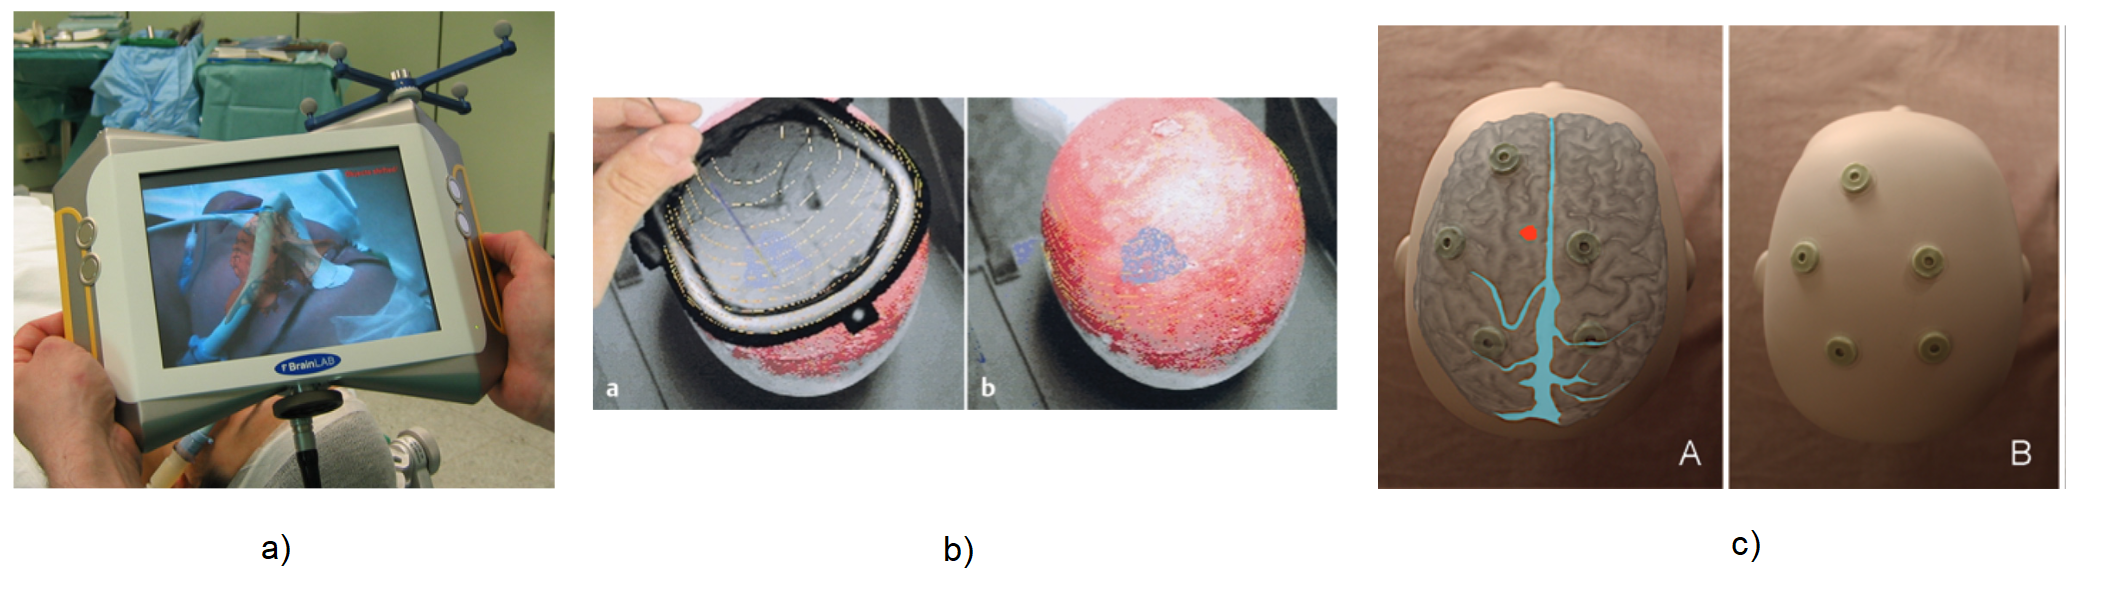
\includegraphics[width=0.9\linewidth]{images/relatedMedicine.png}
	\caption{Abbildungen verschiedener AR-Systeme zur Visualisierung von MRT-Daten im operativen Kontext. a) Bildschirmanwendung zur Unterstützung von Kiefer-OPs von \cite{MISCHKOWSKI2006478}. b) Augmentierung eines Kopfphantoms durch ein tragbares Display von \cite{Wendt03}. c) Durch einen Projektor augementiertes Kopfphantom zum Einsatz in Gehirn-OPs von \cite{Tabrizi15}.}
	\label{img:relatedMed}
	\source{Die Bilder wurden aus den jeweiligen Arbeiten übernommen.}
\end{figure}
\FloatBarrier

Der Einsatz von AR-Anwendungen während einer Operation wird auch von anderen Arbeiten untersucht.
Die Vorgehensweise zur Entwicklung einer solchen Anwendung, sowie die sinnvolle Visualisierung der Bilddaten werden von \cite{grimson99} beschrieben. Einen Überblick über Techniken, die bildgestützte Operationen ermöglichen, liefern \cite{KerstenOertel2013TheSO}.

\cite{Wendt03}, \cite{Maurer01} sowie \cite{fuchs98} entwickeln eine AR-Anwendung für ein tragbares Display, die MRT-Bilder bzw. Bilder einer Laparoskopie bei Eingriffen auf den Patienten projiziert. Die Anwendungen der ersten beiden Arbeiten wurden mit Bildern des Gehirns an einem Kopfphantom getestet.

\cite{MISCHKOWSKI2006478} untersuchen eine bildschirmbasierte AR-Anwendung, die bei Kieferoperationen zum Einsatz kommt. Mit Hilfe der Anwendung kann der Eingriff geplant werden und während der Operation hilft sie dabei, die Position des Kiefers zu überprüfen. 

\cite{GasquesRodrigues17} untersuchen die Einsatzmöglichkeiten von AR und VR im operativen medizinischen Bereich. Dazu gehört unter anderem die Entwicklung einer AR-Anwendung für die Hololens, die die Ausbildung von Ärzten in Anatomie und Operationen unterstützen soll. 

\cite{Watts17} und \cite{Tabrizi15} stellen ebenfalls eine AR-Anwendung vor, die Bilder auf den Körper des Patienten projiziert. Allerdings wird ein Projektoraufbau verwendet, sodass mehrere Betrachter gleichzeitig die Augmentierung sehen können. Wie in den meisten genannten Arbeiten werden Marker auf dem Patienten angebracht, um das Bild anzupassen.

\cite{Soler04} beschreiben Methoden zur Automatisierung einer dreidimensionalen Visualisierung von MRT-Bildern der Verdauungsorgane. Sowie den Einsatz von AR bei Operationen in diesem Bereich. 

In Abbildung \ref{img:relatedMed} sind die Ergebnisse einiger der eben genannten Arbeiten dargestellt.

\subsection{Visualisierung von medizinischem Bildmaterial}

Neben der Entwicklung von AR-Sytemen, die währen eines Eingriffs verwendet werden können, steht im Fokus vieler Arbeiten die Möglichkeiten der dreidimensionalen Visualisierung der menschlichen Anatomie. Indem ein realitätsgetreues Abbild eines Organs erzeugt wird, können Diagnosen und Behandlungsmöglichkeiten erleichtert werden.

% Lesen, Referenzen?
\cite{Mangina17} stellen einen Ansatz zur Erzeugung dreidimensionaler Modelle des Herzens vor, um diese zu Lernzwecken und zur Vorbereitung auf Operationen zu verwenden. Um den Nutzen der 3D-Modelle zu maximieren werden sie in einer AR- und VR-Anwendung platziert. Die Daten die dem Modell zugrunde liegen stammen aus einem MRT-Scan. Zur Implementierung der Anwendungen wurde die Spiele-Engine \textit{Unity} von \cite{unity} verwendet.
Ziel der Anwendung ist es eine interaktive Lernerfahrung zu schaffen, die es dem Nutzer ermöglicht das Herz in seine verschiedenen Komponenten zu zerlegen. Für diesen Anwendungsfall wird ein Mesh des Organs benötigt, das seine Oberfläche abbildet. Die inneren Strukturen sind dabei irrelevant.
Auf Grund der Notwendigkeit eines Meshs wurde der Marching-Cubes Algorithmus zu dessen Erzeugung eingesetzt. Dieser wird in Kapitel \ref{grundlagen} erläutert.
\cite{Mangina17_2} untersuchen die Möglichkeiten zur Erzeugung eines 3D Models aus MRT-Daten genauer.

Ein weiter Ansatz zur Erzeugung von 3D-Modellen des Herzens wird von \cite{SORENSEN2001193} beschrieben. Hier soll das Modell ebenfalls in eine VR-Anwendung integriert und von Ärzten als Vorbereitung auf eine Operation genutzt werden. 
Auch hier soll ein Mesh des Organs erzeugt werden. Die Generierung soll dabei möglichst automatisierbar sein.  Hierzu werden zuerst die Konturen aus den MRT-Bildern extrahiert. Dies resultiert in ein Gitter aus Konturen die dann algorithmisch durch Polygone verbunden werden. 
Für die Anwendung, in der das Modell dargestellt wird wurde ein damals erhältliches VR-System eingesetzt, das mit einem tragbaren Display und zwei Controllern funktionierte. 
Durch die Controller wurde eine eine einfache aber intuitive Interaktion umgesetzt. Der Nutzer kann das Modell Vergrößern und rotieren.  

Neben diesen Arbeiten gibt es noch viele weitere, die sich insbesondere mit der dreidimensionalen Visualisierung von MRT-Daten befassen. Oft werden dafür Volume Rendering Verfahren verwendet. Beispiele für Umsetzungen dieser Art werden im Abschnitt \ref{volumeRenderingImplementierung} beschrieben.

%-------------------------------------------------------------
\section{Magnetresonanztomographie}
\label{mrt}												 %
%-------------------------------------------------------------

Magnetresonanztomographie (MRT) ist ein bildgebendes Verfahren, das auch Kernspintomografie genannt wir. Es wird in der Radiologie verwendet, um Abbildungen innerer Organe zu erzeugen. Während der Durchführung einer MRT wird der Patient in ein MRT-System geschoben, das einer großen Röhre gleicht. Er sollte sich für die Dauer des MRTs möglichst wenig bewegen, um klare Bilder zu erhalten.
Es gibt offene und geschlossene MRT-Systeme. Offene Systeme haben die Form eines C, das den Patienten umgibt und werden daher auch C-Systeme genannt. In einem geschlossenen, wie es in Abbildung \ref{img:mri} zu sehen ist, ist der Patient dagegen vollständig von einer Röhre umgeben. Die Bildqualität ist bei geschlossenen Systemen deutlich besser.

Im folgenden wird die Funktionsweise eines MRT-Scans erläutert, diese wurde von \cite{weishaupt09} beschrieben.

\begin{figure}[!htb]
	\centering
	%https://www.flickr.com/photos/11304375@N07/3081315619/
	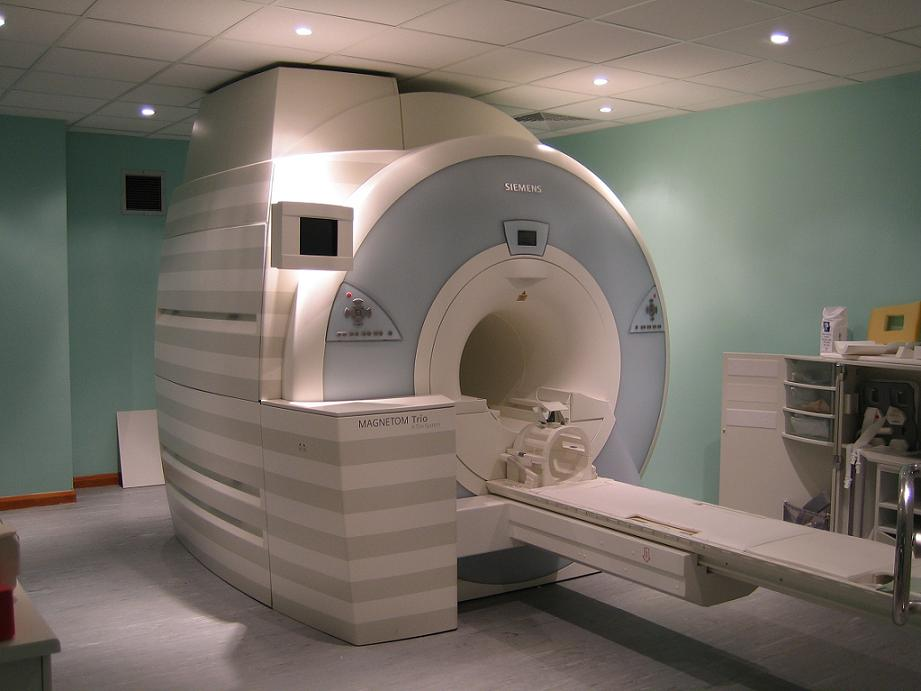
\includegraphics[width=0.5\linewidth]{images/mri.jpg}
	\caption{Ein geschlossenes MRT-Gerät. Auf die Liege im vorderen Bereich legt sich ein Patient, der dann während des Scans in die Röhre geschoben wird. }
	\label{img:mri}
	\source{Übernommen von: https://www.flickr.com/photos/11304375@N07/3081315619/}
\end{figure}
\FloatBarrier

\subsection{Physikalische Grundlagen}

Um die inneren Organe eines Patienten zu visualisieren, werden kleinste Teilchen seines Körpers in Bewegung versetzt, die gemessen werden kann. Im Falle einer MRT handelt es sich dabei um Wasserstoffprotonen. Diese haben eine Eigendrehung um sich selbst, den sogenannten Kernspin. Durch ihre positive Ladung, die durch den Kernspin in Bewegung ist, besitzen die Protonen weiterhin ein eigenes Magnetfeld, welches messbar ist. 
Während einer MRT wird mit einer Hochfrequenz-Spule (HF-Spule), die in dem MRT-System verbaut ist, um den Körper des Patienten ein Magnetfeld erzeugt. Die Kernspin-Achsen der Wasserstoffprotonen richten sich an diesem aus. Anschließend wird in das Magnetfeld ein Hochfrequenzimpuls, die Larmorfrequenz, eingestrahlt. Durch diesen Impuls findet eine Synchronisation der Protonen statt, wobei einige um 180° gedreht werden. Kurz danach laufen die Protonen wieder auseinander und richten sich wieder am Magnetfeld aus. 
Dadurch, dass alle Protonen in dieselbe Richtung zeigen (phasengleich sind), verstärken sie gegenseitig das Signal, dass sie abgeben. Das Signal wird schwächer, sobald sie wieder auseinander laufen (Dephasierung).
Die Zeit, die die Protonen brauchen, um sich wieder am Magnetfeld auszurichten wird als Relaxtionzeit bezeichnet. Dabei wird zwischen T1- und T2-Relaxtion unterschieden.
Die Relaxionszeit ist dabei abhängig von der Zusammensetzung des umgebenden Gewebes. Das gemessene MR-Signal, das durch diese beeinflusst wird, ist also für verschiedene Gewebearten verschieden stark.

\subsection{Erfassung dreidimensionaler Daten}

Mit dem eben beschriebenen Verfahren werden jeweils Werte auf der XY-Ebene erfasst. Um dreidimensionale Daten zu erhalten wird diese XY-Ebene entlang der Z-Achse Verschoben. Der Körper des Patienten wird auf diese Weise in einzelne Schichten unterteilt, von denen jede ein zweidimensionales Bild ist.
Diese Unterteilung in Schichten wird erreicht, indem weitere Spulen verwendet werden, die ein zusätzliches Magnetfeld (Gradientenfeld) erzeugen, welches das erste Magnetfeld inhomogen macht. Dementsprechend fällt es zu einer Seite hin ab, was sich durch einen Gradienten, den Z-Gradienten, beschreiben lässt. So kann jeder Z-Schicht eine bestimmte Stärke im Magnetfeld zugewiesen und einzelne Schichten durch die Verwendung bestimmter Frequenzen angeregt werden. In Abbildung \ref{img:zGradient} ist schematisch dargestellt, wie die Schichten entlang des Z-Gradienten hintereinander liegen und eine von ihnen angeregt wird.
Es wird immer nur eine Schicht auf einmal gescannt und verarbeitet.

\begin{figure}[!htb]
	\centering
	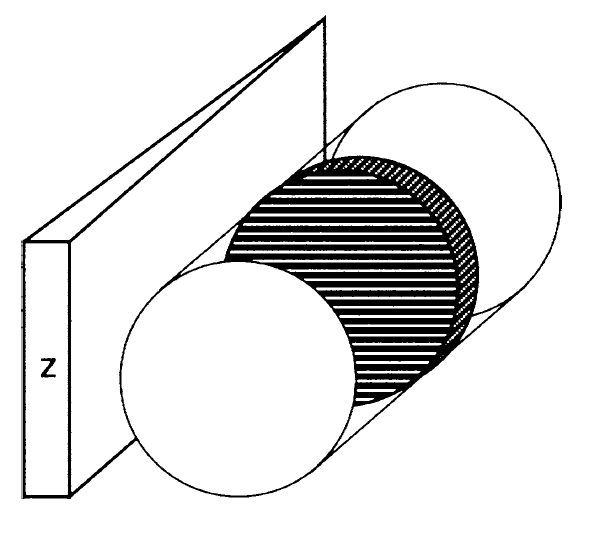
\includegraphics[width=0.3\linewidth]{images/zGradientMrt.png}
	\caption{Darstellung der Schichten während eines MRT-Scans. Links ist der abfallende Z-Gradient zu sehen, daneben drei verschiedene Schichten (Ellipsen). Durch das inhomogene Magnetfeld, kann genau eine Schicht mit einer bestimmten Frequenz angeregt werden. Die ausgewählte Schicht ist hier schraffiert.}
	\label{img:zGradient}
	\source{Übernommen von: \cite{weishaupt09}}
\end{figure}
\FloatBarrier

Die X- und Y-Werte einer Schicht repräsentieren allerdings nicht, wie bei einem Bild Koordinaten, die der Anordnung der jeweils betrachteten Punkte in der Welt entsprechen. Stattdessen bildet der X-Wert die Frequenz und der Y-Wert die Phase ab. Wie für den Z-Wert werden auch hier Gradienten gebildet und auf das Magnetfeld gelegt. Der X-Gradient verläuft von links nach rechts und sorgt dafür, dass die Larmorfrequenz in dieser Richtung zunimmt, sodass die jeder Punkt seine eigene Frequenz hat. Der Y-Gradient, der senkrecht verläuft, beeinflusst auf dieselbe Weise die Phasen einer Schicht. Er wird dabei nur kurz nach dem Einstrahlen des Hochfrequenz-Impulses eingeschaltet, wenn sich die Protonen bereits ausgerichtet haben.

Für jeden Punkt gibt es also eine Magnetfeldstärke (Z), eine Frequenz (X) und eine Phase (Y). Diese Werte aller Punkte werden in einer Matrix gespeichert, die K-Raum genannt wird. In dieser Rohdatenmatrix sind Kontrastwerte und Bilddetails räumlich sortiert. Mit Hilfe einer Fouriertransformation werden sie in lesbare Bilddaten umgewandelt, die die entsprechenden Organe schichtenweise abbilden. 
Die eben erläuterte Erfassung der MRT-Daten wurde von \cite{weishaupt09} beschrieben.

\subsection{Abgrenzung zur Computer-Tomographie}

Eine von der Durchführung ähnliche Methode zur Abbildung des Körperinneren, ist die Computer-Tomographie (CT). Werden die Organe in einer MRT durch magnetische Stimulation ihrer Protonen sichtbar gemacht, wird er Patient bei einer CT schichtenweise geröntgt. D.h. sein Körper wird mit Röntgenstrahlung beschossen, die je nach Gewebe, auf das sie treffen unterschiedlich stark abgeschwächt werden, was anschließend gemessen wird. Die so entstandenen Querschnitte des Körpers werden anschließend mit Hilfe eines Computers zu einem dreidimensionalen Bild zusammengesetzt. \cite{ct1}

Die CT ist deutlich kürzer als eine MRT. Deshalb wird sie oft bei Notfällen verwendet. Allerdings wird der Patient dabei auch der Belastung von radioaktiver Strahlung ausgesetzt, die stärker ist als beim normalen Röntgen. Außerdem können Weichteile mit einer MRT besser darstellt werden. \cite{ct2}
Auf die Einsatzbereiche von CT und MRT im Bezug auf Schlaganfälle wird in Abschnitt \ref{schalganfaelleMRT} eingegangen.

Beide Verfahren liefern Volumendaten als Ergebnis und können demnach in Folgeschritten ähnlich verarbeitet werden.

\pagebreak
\subsection{Medizinische Bilddatenformate}
\label{datenformate}
 
Im medizinischen Bereich gibt es spezielle Datenformate zum Speichern von MRT-Bildern. Da mARt MRT-Bilder visualisiert, werden an dieser Stelle einige relevante Dateiformate vorgestellt. Dazu gehören das NIfTI-Format (Neuroimaging Informatics Technology Initiative) sowie das DICOM-Format (Digital Imaging and Communications in Medicine), welches neben den Bildern z.B. auch Patientendaten speichert. Beide Formate wurden von \cite{Larobina13} beschrieben.

Das NIfTI-Format wurde 2003 von der Data Format Working Group (DFWG) als Alternative zum vorherigen Analyze 7.5-Format entwickelt, das Probleme mit der Orientierung der Daten aufweist. Durch fehlende Informationen, wie die Daten im Raum liegen ist oft unklar, welche die rechte und welche die linke Gehirnhälfte ist. Deshalb wird im NIfTI-Format im Header festgelegt, wie die Koordinaten der Voxel auf Weltkoordinaten abgebildet sind. Beide Formate werden im Bereich des Neuroimaging verwendet.
Bilderinformationen werden bei ersterem in einer einzigen Datei mit der Endung .nii gespeichert, während Analyze 7.5 die Daten in zwei verschiedenen Dateien ablegt: Einer Header-Datei und einer, die die Volumendaten enthält. Während die erste Version des NIfTI-Formats noch mit dem Analyze-Format bitweise kompatibel war, ist es die zweite nicht mehr. 
 
% https://brainder.org/2012/09/23/the-nifti-file-format/

DICOM bezeichnet nicht nur das Dateiformat in dem medizinische Bilder gespeichert werden, sondern  legt auch ein Kommunikationsprotokoll zum Austausch von medizinischen Daten fest. Der DICOM-Standard wird in den meisten medizinischen Einrichtungen verwendet, um medizinische Bilddaten zu speichern und auszutauschen.
%https://hpi.de/fileadmin/user_upload/fachgebiete/meinel/papers/Old_Source/TR_Med_Bildverarbeitung.pdf
Wie bereits erwähnt, speichert eine DICOM-Datei neben den Bilddaten weitere Informationen. Dazu können eine ID oder der Patientenname zählen, die als Attribute des DICOM-Objektes hinterlegt werden. Die Idee dahinter ist, dass die Bilder ohne Metadaten keine Bedeutung haben. 

MRT-Bilder werden außerhalb des medizinischen Umfelds allerdings auch in anderen Formaten gespeichert. 
Ein Beispiel dafür ist das PVM-Format, das zum Speichern von volumetrischen Daten genutzt wird. Das Format geht davon aus, dass das Volumen aus quadratischen Voxeln besteht und enthält die Voxelwerte und Größeninformationen über das Volumen. Es wird von \cite{pvm} beschrieben.
% http://paulbourke.net/dataformats/pvm/

Die Daten können weiterhin in herkömmlichen Bildformaten, wie JPEG oder PNG gespeichert werden. Dabei entspricht dann eine Bilddatei einer Schicht des Scans. 
 
%\cite{graham05} beschrieben DICOM Format und DICOM Viewer.
%16 bit int images, pvm ? Standart?

%------------------------------------------------------
\section{Volumendaten}
\label{volumeData}					  	  %
%------------------------------------------------------

Ein wichtiger Aspekt dieser Arbeit ist die dreidimensionale Visualisierung von MRT-Daten. Deshalb soll an dieser Stelle auf einige grundlegende Aspekte und Begriffe im Zusammenhang mit Volumendaten eingegangen werden.

Da das Gehirn durch einen MRT-Scan dreidimensional erfasst wird, liegen die MRT-Daten als Volumendaten vor. Die Daten werden durch ein Skalarfeld repräsentiert. Ein Skalarfeld ist eine Sammlung von Skalarwerten, die in einem Raum verteilt sind. Durch eine Funktion kann jedem Punkt im Raum ein Skalarwert zugewiesen werden. Im Fall von Volumendaten handelt es sich um ein dreidimensionales Skalarfeld. D.h. die Skalarwerte sind innerhalb eines Quaders angeordnet und für jeden Skalarwert existieren X-, Y- und Z-Koordinaten, die dessen Position beschreiben. 
Diese Punkte, aus denen sich der Volumen-Quader zusammensetzt, werden auch Voxel genannt. Ähnlich wie Pixel in zweidimensionalen Bildern stellen sie die kleinsten Teile in einem Volumen dar. 
Die Skalarwerte werden auch als Isowerte des Volumens bezeichnet. Bei MRT-Daten bildet jeder Wert eine Graustufe mit einer Farbauflösung von 256 Stufen ab. 
Über das Volumen verteilt haben benachbarte Werte oft ähnliche Isowerte. Eine Gruppe dieser Werte wird als Isofläche bezeichnet. Isoflächen innerhalb eines Volumens entsprechen meist tatsächlichen Oberflächen des darzustellenden Objektes. Durch den Vergleich benachbarter Werte ist es möglich Oberflächen von Objekten zu ermitteln. Der Marching-Cubes Algorithmus, der in Abschnitt \ref{marchingCubes} erläutert wird, wendet diesen Vergleich an. 
Volumendaten werden oft in 3D-Texturen gespeichert. Diese verfügen im Gegensatz zu 2D-Texturen über eine zusätzliche Z-Komponente. 

Die Verfahren zur dreidimensionalen Visualisierung von MRT-Daten werden von \cite{Zhang10} in drei Bereiche geteilt: Multiplanar Reformation, Surface Rendering, und (direct) Volume Rendering. In den folgenden Abschnitten werden verschiedene Verfahren des Volume Renderings sowie eine prominente Surface Rendering Technik erläutert.

%------------------------------------------------------
\section{Volume Rendering}							  %
%------------------------------------------------------

Wie in Abschnitt \ref{motivation} erläutert, sollen MRT-Bilder, die ein Neurologe untersucht in mARt als dreidimensionales Volumen dargestellt werden. Volume Rendering bezeichnet die Darstellung eines Volumens, das meist durch ein Skalarfeld repräsentiert wird, als Projektion auf ein zweidimensionales Bild. MRT-Bilder, die in Graustufen vorliegen bilden ein solches Skalarfeld. 

Dadurch, dass das Volumen aus Voxeln gebildet wird, gibt es keine Oberfläche, die das abzubildende Objekt beschreibt. Die Darstellung erfolgt deshalb anhand eines optischen Modells. Jedem Wert im Datensatz werden dazu optische Eigenschaften zugewiesen, im Allgemeinen Farbe und Opazität. %Indem Strahlen durch das Volumen geschossen werden, werden diese Eigenschaften miteinander verrechnet, was schließlich zur Abbildung des gesamten Volumen führt. Diese Technik wird im Abschnitt \ref{rayCasting} genauer beschrieben.
Die einzelnen Voxel werden abhängig vom Blickwinkel des Nutzers durch eine Berechnungsvorschrift, die vom jeweiligen Renderdingverfahren bestimmt wird, auf eine zweidimensionale Ebene abgebildet.
Die optischen Eigenschaften eines Voxels sind abhängig von seinem Isowert, sowie der verwendeten Transferfunktion und dem Shading. 
Im Folgenden werden grundlegende Bestandteile des Volume Rendering erläutert.%Techniken, sowie verschiedene Verfahren der Umsetzung des Volume Rendering erläutert.

\cite{Kaufman03}
\cite{kniss02}
\todo{Was ist mit diesen Referenzen?}

\subsection{Klassifikation}
\label{klassifikation}

Die Klassifikation von Voxeln nach \cite{Hadwiger06} bestimmt deren optische Eigenschaften in Abhängigkeit zu ihrem Isowert. Die Eigenschaften repräsentieren die Aufnahme und Abgabe von Licht eines einzelnen Voxels. Die Abgabe von Licht manifestiert sich in der Farbe eines Voxels. Die Aufnahme äußert sich in dem Grad der Opazität. Durch die Unterschiede in Farbe und Opazität einzelner Voxel werden verschiedene Bereiche, wie z.B. Gewebestrukturen voneinander unterscheidbar. Die Qualität des gerenderten Bildes hängt zu einem großen Teil von der Klassifikation ab. Oft wird eine Transferfunktion verwendet, um Voxel zu klassifizieren, durch die jedem Isowert ein Opazitäts- und Farbwert zugewiesen wird. Auf diese wird im folgenden Abschnitt näher eingegangen. 
Für die Darstellung der Daten in mARt werden diese ebenfalls klassifiziert. An dieser Stelle soll ein Überblick über verschiedene Klassifikationen gegeben werden.

Das Ergebnis einer Klassifikation hängt von dem Zeitpunkt ab zu dem diese durchgeführt wird. Sie kann vor oder nach der Interpolation der Volumendaten durchlaufen werden.
Die Daten müssen interpoliert werden, da das Volumen, wie mehrfach beschrieben, in einzelnen Werten vorliegt. Der Raum zwischen diesen Werten ist nicht definiert. Um ein zusammenhängendes Volumen darstellen zu können muss also eine Interpolation zwischen den Werten stattfinden. Diese geschieht während des Rasterisierungsschrittes der Grafikpipeline.

Werden die Voxel vor dieser Interpolation klassifiziert, wird dies als Pre-Klassifikation bezeichnet. Dabei werden jedem Isowert die entsprechenden Eigenschaften zugewiesen. Die zwischen den Voxeln bestehenden Lücken werden aufgefüllt, indem zwischen den Farb- und Opazitätswerten interpoliert wird. 
Im Gegensatz dazu werden bei der Post-Klassifikation zuerst alle Skalarwerte durchlaufen und der Bereich zwischen ihnen durch Interpolation der Isowerte überbrückt. Erst danach werden den Werten durch die Klassifikation Eigenschaften zugewiesen. Der Unterschied besteht also darin, ob die Erzeugung von neuen Werten, die die vorhandenen verbinden auf Basis der Voxelwerte oder der Werte ihrer Eigenschaften stattfindet. 

Obwohl die Vorgehensweisen also beinahe gleich sind, führen sie doch zu deutlich unterschiedlichen Ergebnissen. Die Interpolation der Voxeleigenschaften bei der Pre-Klassifikation führt zu Artefaktbildung, da die später ermittelten Eigenschaftswerte lediglich gestreckt werden, ohne dass die Formen des Volumens beachtet werden. Bei der Post-Klassifikation werden die fehlenden Daten anhand der Struktur des Objektes erzeugt. Dies führt zu einer deutlich klareren Darstellung des Volumens. Der Vergleich ist in Abbildung \ref{img:prepost} veranschaulicht.

\todo{Bild ersetzen}
\begin{figure}[!htb]
	\centering
	%http://schorsch.efi.fh-nuernberg.de/roettger/index.php/VolumeRendering/Pre-AndPost-Classification
	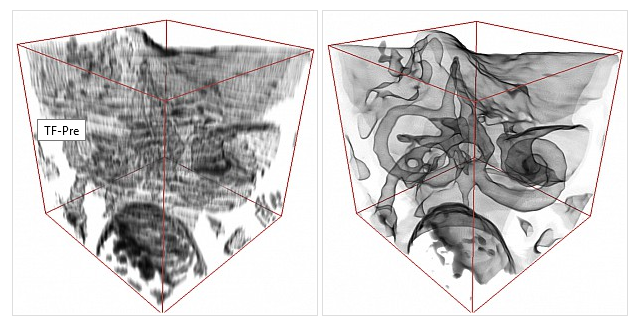
\includegraphics[width=0.7\linewidth]{images/prepostclassification.png}
	\caption{Vergleich zweier Volumen Renderings mit unterschiedlicher Klassifizierung. Durch die Verwendung von Pre-Klassifikation (links) entstehen Artefakte. Die Post-Klassifikation (rechts) liefert eine bessere Darstellung des Volumens.}
	\label{img:prepost}
	\source{Übernommen von: http://schorsch.efi.fh-nuernberg.de/roettger/index.php/VolumeRendering/Pre-AndPost-Classification}
\end{figure}
\FloatBarrier

Aber auch bei der Verwendung einer Post-Klassifikation können Artefakte entstehen.
Um das Volumen darzustellen, werden Proben einzelner Voxel genommen und ihre Eigenschaftswerte in Abhängigkeit zu dem verwendeten Renderingverfahren miteinander verrechnet. 
Die Frequenz, in denen die Werte geprüft werden, kann dabei variieren. Ist der Abstand zwischen zwei Voxeln zu groß, kann es dazu kommen, dass Wertveränderungen, die zwischen diesen liegen nicht erfasst werden, wodurch Artefakte entstehen. 
Um dem entgegen zu wirken, kann die Abtastfrequenz erhöht werden. Dies resultiert allerdings in einen höheren Rechenaufwand, der das Rendering verlangsamt.
Eine alternative Lösung ist die Verwendung einer Pre-Integrierten Klassifikation.
Um alle Werte zwischen zwei Voxeln zu erfassen, wird hierbei nicht nur der Wert eines Voxels betrachtet, sondern der Bereich zwischen diesem und dem nächsten, der abgetastet werden soll. 

Das Volumen wird somit in Segmente aufgeteilt, die jeweils durch einen vorderen und hinteren Punkt begrenzt werden. Für jedes Segement und damit für jeden Abtastpunkt, wird durch Bildung eines Integrals sowohl der Opazitäts- als auch der Farbwert approximiert. 
Die Errechnung des Opazitätwertes $a_i$ des  $i$-ten Abtastpunktes lässt sich wie folgt beschreiben:

\begin{align}
   a_i = 1-exp\left ( \int_{id}^{(i+1)d)} \kappa\left ( s(\mathbf{x}(\lambda)) \right ) d\lambda  \right )
\end{align}

Wobei:
\begin{itemize}
\item $\lambda$ 			: aktueller Punkt auf dem Strahl
\item $\mathbf{x}(\lambda)$ : Berechnung der Koordinaten des Volumens für $\lambda$
\item $s(x)$				: Bestimmung der Isowerte
\item $\kappa(x)$			: Transferfunktion für Opazität
\item $d$					: Abstand zwischen Abtastpunkten
\end{itemize}
 
%Durch die Funktion  $\mathbf{x}(\lambda)$ werden die Koordinaten des Volumens berechnet, an denen der Punkt sich befindet. $\lambda$ repräsentiert dabei den aktuellen Punkt auf dem Strahl. 
%Die Koordinaten werden $s(x)$ übergeben, wodurch die Isowerte an dieser Stelle bestimmt werden. $\kappa(x)$ ist die Transferfunktion für die Opazitätwerte, die anschließend noch mit dem Abstand zwischen den Abtastpunkten $d$ und $\lambda$ multipliziert wird.

Der Integral der Transferfunktion beschreibt den Flächeninhalt des Bereichs unter ihr, im Intervall von $id$ bis $(i+1)d$. Veränderungen der Funktion zwischen diesen Punkten wirken sich auf die durch das Integral beschriebene Fläche aus. 
Der Flächenwert dient als Exponent einer Exponentialfunktion, deren Ergebnis anschließend von $1$ abgezogen wird. Dadurch wird der Integralwert in einen Bereich zwischen $0$ und $1$ überführt. 
Die Berechnung der Farbe erfolgt auf dieselbe Weise.
Wie in Abschnitt \ref{3dDarstellung} erläutert wird, wird das Volume Rendering für mARt im Fragment Shader durchgeführt. Dementsprechend handelt es sich dabei um eine Post-Klassifikation.

\subsection{Transferfunktion}

Transferfunktionen nach \cite{Fernando04} bilden den Isowert auf beliebige Eigenschaften ab, wie  Farbe und Opazität.  Unterschiedliche Gewebearten können auf diese Weise eingefärbt oder ausgeblendet werden. In der Umsetzung besteht eine Transferfunktion meistens aus einer Textur, die als Look-Up-Tabelle verwendet wird. Daraus kann für jeden Isowert eine Farbe und Opazität gelesen werden. Die Textur kann dabei eindimensional sein, wenn als Index lediglich der Isowert des Voxels verwendet wird. Für eine bessere Unterscheidung der Gewebe eines Objektes können allerdings auch multidimensionale Transferfunktionen eingesetzt werden. Hierbei werden neben dem Isowert z.B. auch der Betrag des Gradienten des jeweiligen Voxels als Koordinaten für die Transfertextur verwendet. In Abbildung \ref{img:transferfunction} ist der Unterschied zwischen der Verwendung von ein- und zweidimensionalen Transferfunktionen verdeutlicht. Der Zugriff auf die Transferfunktion erfolgt genauso wie bei anderen Texturen. Im Codebeispiel \ref{lst:transfer} ist demonstriert, wie in einem Shader auf die 3D-Textur des Volumens und die 1D-Textur der Transferfunktion zugegriffen wird. 

\begin{listing}[!htb]
\begin{minted}[mathescape,
               linenos,
               numbersep=5pt,
               gobble=2,
               frame=lines,
               framesep=2mm]{csharp}
void main(sampler3D _Volume,
          sampler1D _TransferTexture,
          float3 texCoord : TEXCOORD0,
          float4 color : COLOR)
{
  // Der Isowert des Volumens wird für die aktuelle Position ausgelesen
  float isoValue = tex3D(_Volume, texCoord);
  // Die Farbe des Volumens wird für die aktuelle Position ausgelesen
  color = tex1D(_TransferTexture, isoValue);
}
\end{minted}
\caption{Aus einer 3D-Textur wird ein Isowert gelesen. Dieser wird verwendet, um aus einer 1D-Transfertextur die entsprechende Farbe auszulesen. Übernommen von: \cite{Fernando04}}
\label{lst:transfer}
\end{listing}
\FloatBarrier

Eine gute Transferfunktion zu implementieren ist sehr schwierig, da die korrekten Werte oft nur durch Ausprobieren gefunden werden können und von dem jeweiligen Datensatz abhängen. Teilweise werden Widgets eingesetzt, die es dem Nutzer erlauben eine Transferfunktion zu erstellen, die in Echtzeit auf ein gerendertes Volumen angewandt wird.
\cite{salama06} und \cite{Knig99} beschreiben die Entwicklung von Benutzeroberflächen zur Erstellung von Transferfunktionen.
Die Verwendung einer Transferfunktion ist Teil der Klassifikation von Voxeln, da über die Transferfunktion definiert ist, welche Isowerte welchem Gewebe entsprechen.

\begin{figure}[!htb]
	\centering
	%http://developer.download.nvidia.com/books/HTML/gpugems/gpugems_ch39.html
	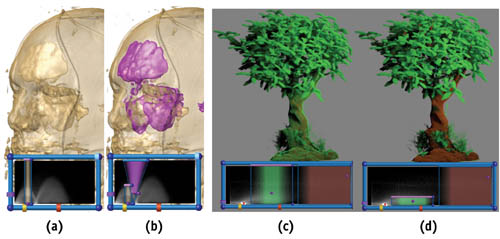
\includegraphics[width=0.7\linewidth]{images/transferfunction.jpg}
	\caption{Abbildung zweier gerenderter Volumen und der jeweils dafür verwendeten Transferfunktion. In den Darstellungen a) und c) wurde eine eindimensionale Transferfunktion verwendet. b) und c) benutzen zweidimensionale Tranfserfunktionen, wodurch verschiedene Bereiche des Volumens anders eingefärbt sind.}
	\label{img:transferfunction}
	\source{Übernommen von: \cite{Fernando04}}
\end{figure}
\FloatBarrier


\subsection{Beleuchtung}
\label{beleuchtung}

Um dem gerenderten Objekt einen möglichst plastischen Eindruck zu verleihen und es somit realistischer aussehen zu lassen, ist es sinnvoll dieses zu beleuchten. 
%Die Beleuchtung wird in der Regel durch einen Shader implementiert.
Für jeden Voxel wird dabei einzeln die Auswirkung der Beleuchtung ermittelt, nachdem die  Transfertextur angewendet wurde, sodass dessen Eigenschaften zusätzlich zu dieser verändert werden. Es können verschiedene Modelle zur Beleuchtung verwendet werden. Außerdem ist zwischen lokaler und globaler Beleuchtung zu unterscheiden. Die Beleuchtung von Volumen wurde von \cite{Fernando04} erläutert.

Die lokale Beleuchtung betrachtet nur die Beziehung des Lichtes zu dem Objekt. Dabei werden Beleuchtungseffekte, wie Schatten oder indirekte Beleuchtung ignoriert. Zudem ist das Beleuchtungsmodell auf Oberflächen ausgelegt und nicht auf ein Volumen. 

Eine realistischeres Ergebnis liefert daher die globale Beleuchtung, bei der das Objekt Schatten wirft und indirekt beleuchtet wird. 
Um Schatten im Volumen darzustellen, muss bestimmt werden wie viel Licht bei einem Voxel ankommt, nachdem das Licht andere Voxel passiert hat und dadurch abgeschwächt wurde. 
Dazu könnte ein Schattenvolumen erstellt werden, indem jeder Voxel aus Sicht des Lichts gerendert wird, welches mit den Werten aus der Transfertextur verrechnet wird. Dieses Vorgehen ist allerdings unperformant und liefert keine guten Ergebnisse.

Stattdessen wird das Volumen durch Texture Slicing in Schichten unterteilt \cite{Hadwiger06}. Jede Schicht wird dann jeweils aus Sicht der Kamera und des Lichtes gerendert. Jedes der beiden gerenderten Bilder wird in einem 2D-Textur-Buffer gespeichert. 
Die Lage der Schichten wird durch die Winkelhalbierende des Blickrichtungsvektors und des Lichtrichtungsvektors bestimmt. Dadurch treffen beide Vektoren im selben Winkel auf die Schichten. Abhängig von dem Skalarprodukt der Vektoren kann auch die Inverse des Blickwinkels verwendet werden. Das Skalarprodukt bestimmt außerdem, ob die Schichten aus Kamerasicht von hinten nach vorne oder von vorne nach hinten durchlaufen werden, während für das Licht immer von vorne nach hinten gerendert wird.
Die Position der Vektoren und der winkelhalbierenden Schicht ist in Abbildung \ref{img:halfAngleSlice} dargestellt.
	
\begin{figure}[!htb]
	\centering
	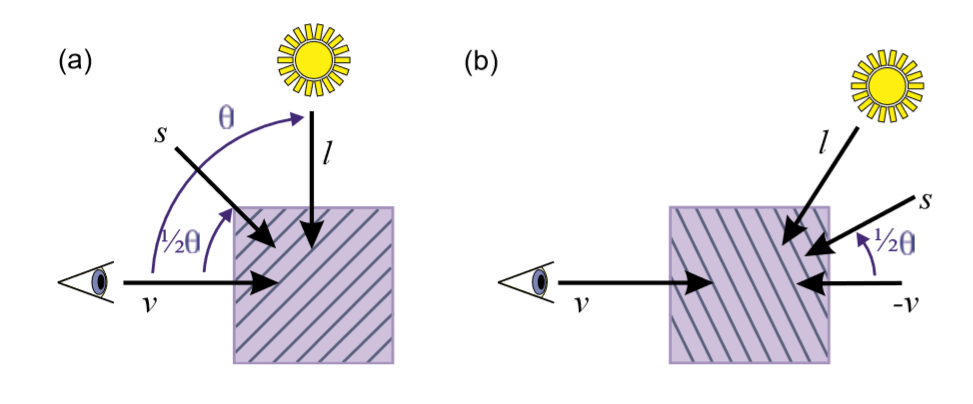
\includegraphics[width=0.7\linewidth]{images/halfAngleSlice.png}
	\caption{Durch Bestimmung der Winkelhalbierenden des Licht- und Kamerarichtungsvektors, wird die Lage der Schichten bestimmt, die sowohl aus Licht- als auch Kamerasicht gerendert werden. Bei einem Skalarprodukt $>=0$ wird der Kameravektor verwendet (a), bei einem negativen Skalarprodukt dessen Inverse (b).}
	\label{img:halfAngleSlice}
	\source{Übernommen von: \cite{Hadwiger06}}
\end{figure}
\FloatBarrier

Jede Schicht wird dann zuerst aus Sicht der Kamera gerendert. Die aus Lichtsicht gerenderte vorhergehende Schicht ist dabei bereits bekannt. So kann jeder Punkt des Kamera-Textur-Buffers mit jedem des Licht-Textur-Buffers der vorherigen Schicht verrechnet werden. Dabei wird durch den Wert des Kamera-Buffers die Farbe und Opazität aus der Transferfunktion gelesen. Die entsprechende Farbe wird dann mit dem Wert aus dem Licht-Buffer multipliziert. Die so berechnete Schicht wird wieder in den Kamera-Buffer geschrieben. Dann wird die aktuelle Schicht aus Sicht der Lichtquelle in den Licht-Buffer gerendert, um diesen für die nächste Schicht zu verwenden.
Für jede Schicht wird ein eigener Pass durchlaufen.

Indirekte Beleuchtung entsteht, wenn ein Objekt von Licht getroffen wird, das vorher von woanders reflektiert wurde. Bei einem Volumen beschreibt es dabei in der Regel die Streuung von Licht innerhalb des Volumens. Dabei wird dass Licht, nachdem es auf das Objekt getroffen ist, von dessen Inneren gebrochen, während es in dieses eindringt. Dies ist der Fall bei Objekten aus transluzentem Material, wie z.B. Wachs oder Haut.

\cite{hansen02} stellen ein Shading Modell vor, dass realistisches Rendering von transluzenten Materialien erlaubt.
\todo{Phasenfunktion} 

Die globale Beleuchtung ist somit von der Umsetzung deutlich komplexer, bietet allerdings auch mehr Plastizität und Realismus. Dies wird in Abbildung \ref{img:localGlobalIll} deutlich, in der die Ergebnisse der beiden Vorgehensweisen gegenübergestellt sind.
\cite{Jnsson14} untersuchen derzeit verwendete Beleuchtungsmethoden von Volumen.
\todo{Was untrsuchen die genau?}
\begin{figure}[!htb]
	\centering
	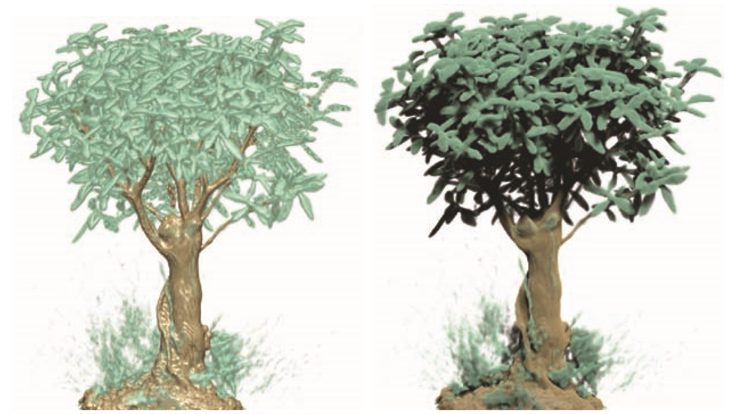
\includegraphics[width=0.7\linewidth]{images/localGlobalIllumination.png}
	\caption{Vergleich zweier Volumen, die mit lokaler Oberflächenbeleuchtung (links) und direkter Beleuchtung und Schatten (rechts) gerendert wurden.}
	\label{img:localGlobalIll}
	\source{Übernommen von: \cite{Hadwiger06}}
\end{figure}
\FloatBarrier

Aufgrund der hohen Komplexität der globalen Beleuchtung, wird im Rahmen dieser Arbeit nur eine lokale Beleuchtung implementiert. 
Hierzu wird in vielen Fällen das Phong-Beleuchtungmodell verwendet und wird auch für mARt implementiert.

% PHONG
Das Modell nach \cite{phong75} setzt sich aus drei Komponenten zusammen: Der ambienten und der diffusen Beleuchtung, sowie der Reflexion. Diese werden aufeinander addiert und ergeben so das Phong-Beleuchtungsmodell. In Abbildung \ref{img:phong} ist zu sehen, wie die einzelnen Komponenten isoliert aussehen und wie sie in Kombination die vollständige Beleuchtung ergeben.
Die folgende Formel beschreibt, wie die Beleuchtung berechnet wird. Die Terme zwischen den $+$-Zeichen stehen für die Berechnungen der genannten Komponenten.

\begin{align}
I = k_{a}+I_{L}k_{d}(\vec{l}\cdot\vec{n})+I_{L}k_{s}(\vec{r}\cdot\vec{v})^n
\end{align}


$I$ ist dabei die Farbe des beleuchteten Punktes, die bei Verwendung einer Transferfunktion durch diese bestimmt wird. $\vec{n}$ ist die Normale und $\vec{l}$ ist der Richtungsvektor zum Licht. $I_{l}$ ist die Intensität des Lichtes. $\vec{r}$ und $\vec{v}$ sind der Reflexionsvektor des einfallenden Lichtes und der Richtungsvektor zur Kamera. Weiterhin setzt sich die Formel aus dem ambienten, diffusen und spiegelndem Koeffizienten $k_{a}$, $k_{d}$ und $k_{s}$ zusammen. Hinzu kommt der Exponent $n$, der die Stärke der Reflexion bestimmt. 

\begin{figure}[!htb]
	\centering
	%https://commons.wikimedia.org/wiki/File:Phong_components_version_4.png
	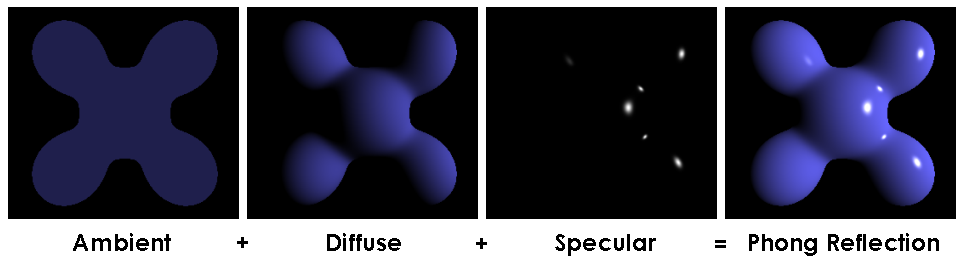
\includegraphics[width=0.7\linewidth]{images/Phong_components_version_4.png}
	\caption{Visuelle Aufteilung des Phong-Beleuchtungsmodells in seine drei Komponenten. Die Farbe pro Pixel wird für jede Komponente einzeln berechnet und die Komponenten schließlich zusammen addiert.}
	\label{img:phong}
	\source{Übernommen von: https://commons.wikimedia.org/wiki/File:Phong\_components\_version\_4.png}
\end{figure}
\FloatBarrier

\subsection{Gradientenberechnung}

Um die in Abschnitt \ref{beleuchtung} erläuterte Beleuchtung umzusetzen, müssen die Normalen der einzelnen Voxel bekannt sein. Da die Voxel allerdings keine Oberfläche bilden, besitzen sie auch keine Normalen. Als Ersatz können stattdessen die Gradienten der Voxel verwendet werden. Diese beschreiben die Wertveränderung in der Umgebung eines Voxels und zeigen dabei auf die Größte Veränderung. Benachbarte Voxel mit ähnlichen Isowerten bilden eine Isofläche, die durch die Gradienten beschrieben wird. 
% ??

Zur Berechnung der Gradienten können verschiedene Verfahren eingesetzt werden. Der Unterschied in der Berechnung liegt vor allem in dem Zeitpunkt zu dem diese ausgeführt werden. Gradienten können entweder vor dem Start des Programmes berechnet werden oder zur Laufzeit. 

%Ist ersteres der Fall werden die Gradienten in den meisten Fällen per Pixel mit Hilfe der Finite-Differenzen-Methode berechnet.
Bei mARt ist ersteres der Fall. Die Gradienten werden dazu per Pixel mit Hilfe der Finite-Differenzen-Methode berechnet \cite{Hadwiger06}.
Dabei wird jeweils die Differenz zwischen dem Isowert eines Voxels und den Voxeln in seiner festgelegten Umgebung gebildet. Dies lässt sich als folgende Formel ausdrücken: 

\begin{align}
\Delta f(x,y,z)\approx \frac{1}{2h}
\left ( \begin{matrix}
f(x + h, y, z) - f(x - h, y, z)\\ 
f(x, y + h, z) - f(x, y - h, z)\\ 
f(x, y, z + h) - f(x, y, z - h)
\end{matrix} \right )
\end{align}

\todo{Convolution?}
%\todo{On´The fly gradientenberechnung}
%\todo{genau vorstellen}
%\todo{Vergleich der versch. formen -> BUCH}

\cite{Correa11} haben verschiedene Methoden zur Bestimmung von Gradienten verglichen.
\todo{Was wird verglichen}
\todo{Segmentierung}

\subsection{Komposition}

Komposition bezeichnet die Verrechnung einzelner Voxelwerte \cite{Fernando04}. Abhängig von der Blickrichtung der Kamera beeinflussen die Eigenschaften eines Wertes das Aussehen des gerenderten Pixels. Um die endgültige Farbe eines Pixels zu erhalten werden die Werte von hintereinander liegenden Voxeln in der Regel aufaddiert. Hierbei ist es von Relevanz, in welcher Reihenfolge die Werte durchlaufen werden. Wird das Volumen von vorne nach hinten durchlaufen, erfolgt die Komposition wie folgt:

\begin{align}
\hat{C}_{i}=(1-\hat{A}_{i-1})C_{i}+\hat{C}_{i-1}
\end{align}
\begin{align}
\hat{A}_{i}=(1-\hat{A}_{i-1})A_{i}+\hat{A}_{i-1}
\end{align}


Wobei $\hat{C}_{i}$ die Farbe und $\hat{A}_{i}$ die Transparenz der Farbe des vordersten Voxels ist.
Sollen die Werte von hinten nach vorne addiert werden, wird dies durch die folgende Formel beschrieben.

\begin{align}
\hat{C}_{i}=C_{i}+(1-\hat{A}_{i})\hat{C}_{i+1}
\end{align}
\begin{align}
\hat{A}_{i}=A_{i}+(1-\hat{A}_{i})\hat{A}_{i+1}
\end{align}

Die Komposition erfolgt pro Voxel am Ende des Renderingprozesses. Die Eigenschaften des Voxels können in dessen Verlauf verändert werden. Beispielsweise durch die Verwendung einer Transferfunktion oder eines Shaders.


\section{Volume Rendering Methoden}

An dieser Stelle werden verschiedene Methoden erläutert, mit denen Volume Rendering umgesetzt werden kann. Die Implementierung dieser Arbeit verwendet das Volume Raycastingverfahren. Es werden allerdings auch andere prominente Methoden beschrieben, um einen Überblick über die Thematik und die Möglichkeit eines Vergleichs zu schaffen.

\subsection{Volumetrisches Raycasting}
\label{rayCasting}

\todo{REFERENZEN}

\begin{figure}[!htb]
	\centering
	%https://de.wikipedia.org/wiki/Datei:Volume_Ray_Casting-de.svg
	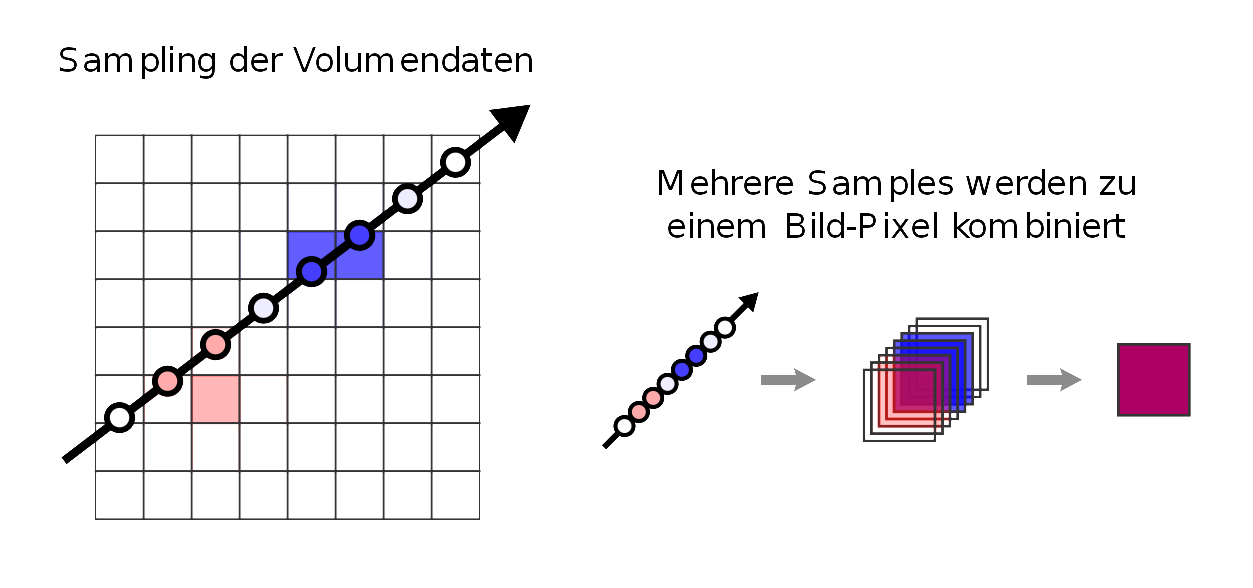
\includegraphics[width=0.7\linewidth]{images/rayCasting.png}
	\caption{Schematische Darstellung des Volume Raycastings. Ein Strahl (Pfeil) durchläuft das Volumen (Würfel). Die Eigenschaften (Farbe und Opazität) jedes Voxels, der passiert wird werden zusammengerechnet, um die Farbe eines Pixels des Renderings zu erhalten.}
	\label{img:rayCasting}
	\source{Übernommen von: https://commons.wikimedia.org/wiki/File:Volume\_Ray\_Casting-de.svg}
\end{figure}
\FloatBarrier

Raycasting ist eine bekannte Renderingmethode, die auch beim Rendering von 3D-Szenen zur Anwendung kommt, die keine Volumendaten enthalten.
Dabei werden von der Position der Kamera für jeden Pixel Strahlen in die Szene geschossen. Für jeden Strahl wird dann errechnet, ob dieser die Oberfläche eines der Objekte in der Szene schneidet. Ist dies der Fall, wird der betreffende Pixel in der Farbe des Objektes eingefärbt, wobei der verwendete Shader diese beeinflusst. Es wird außerdem berücksichtigt, welche Länge der Strahl zu dem Schnittpunkt hat, da nur der Eintrittspunkt relevant ist.

Weiterhin existieren die Techniken Raytracing und Raymarching, die ebenfalls auf der Kollision zwischen Strahlen und Objekten beruhen.
Beim Raytracing werden dabei neben dem ursprünglichen Strahl, der das Objekt trifft noch weitere berechnet, welche vom Treffpunkt des Objekts, abhängig von seiner Oberflächenbeschaffenheit und seinem Material reflektiert und weiter durch die Szene verfolgt werden.
Raymarching ist eine schnellere Version des Raycastings. 
Hier wird der Schnittpunkt von Strahl und Oberfläche nicht genau berechnet. Stattdessen wird entlang des Strahls in kleiner werdenden Abständen jeweils ein einzelner Punkt betrachtet. Für diesen Punkt wird lediglich geprüft, ob er sich bereits innerhalb des Objektes befindet oder nicht. Der erste Punkt, auf den dies zutrifft wird als Schnittpunkt angesehen. Obwohl diese Berechnung weniger genau ist, ist sie schneller als Raycasting.

%Raycasting bzw. Ray-Marching wird auch zum Rendering von Volumen benutzt.
Bei allen Verfahren muss die Oberfläche bzw. die Form des Objektes bekannt sein, um bestimmen zu können, wann der Strahl in sie eintritt. Dies ist bei Volumendaten in der Regel nicht gegeben, da nicht nur das Objekt selbst, sondern auch dessen Umgebung darin gespeichert sind. Weiterhin werden durch die eben beschriebenen Prozesse nur die Oberflächen der Objekte gerendert, nicht aber ihr Inneres.

Hier liegt der Unterschied zum Rendering von Volumen. Volumetrisches Raycasting oder volumetrisches Raymarching vereint die beiden beschriebenen Verfahren. Auch hier werden dabei Strahlen von der Kamera in die Szene geschossen. Um das Volumen zu rendern sind davon nur die Strahlen relevant, die das Volumen treffen. Und auch von dieser Teilmenge wird jeweils nur der Teil des Strahls berücksichtigt, der innerhalb der umgebenden Geometrie liegt. Für jeden Strahl wird deshalb der Ein- und Austrittspunkt errechnet. Innerhalb der Geometrie werden anschließend entlang des Strahls in bestimmten Abständen Voxel betrachtet. Für jeden Voxel wird per Klassifikation ein Farb- und Opazitätswert bestimmt und die Werte werden abhängig von der Komposition von hinten nach vorne oder von vorne nach hinten aufeinander addiert. Die Summen der Werte ergeben so eine dreidimensionale Darstellung des Volumens aus der Sicht der Kamera. Der Vorgang ist in Abbildung \ref{img:rayCasting} veranschaulicht.


\subsection{Texture-Based Volume Rendering}

Beim texturbasierten Rendering von Volumen wird eine dreidimensionale Darstellung erzeugt indem viele Texturen aufeinander geschichtet werden, die dann übereinander geblendet werden. Dazu wird für jede Schicht ein Querschnitt durch das Volumen gemacht, auf den mit Hilfe von Texture Mapping die Textur gerendert wird.
Die Form und Ausrichtung der Querschnitte wird dadurch bestimmt in welcher Form die Volumendaten vorliegen. In Abbildung \ref{img:2D3DTex} wird der Unterschied verdeutlicht. Handelt es sich um zweidimensionale Texturen,  richten sich die Querschnitte am Volumen aus. Innerhalb eines Würfel sind sie also quadratisch. Damit das Volumen aus verschiedenen Blickwinkeln betrachtet werden kann, wird für jede der Hauptsichtachsen ein Stapel mit Texturen erstellt. Zwischen den Stapeln wird gewechselt, sobald sich der Betrachtungswinkel ändert. Dadurch wird verhindert, dass der Betrachter zwischen zwei Texturen hindurchsehen kann, wenn diese annähernd parallel zu seiner Blickrichtung stehen. Dies ist in Abbildung \ref{img:textureBased} dargestellt.

\begin{figure}[!htb]
	\centering
	%https://www.evl.uic.edu/aej/524/lecture06.html
	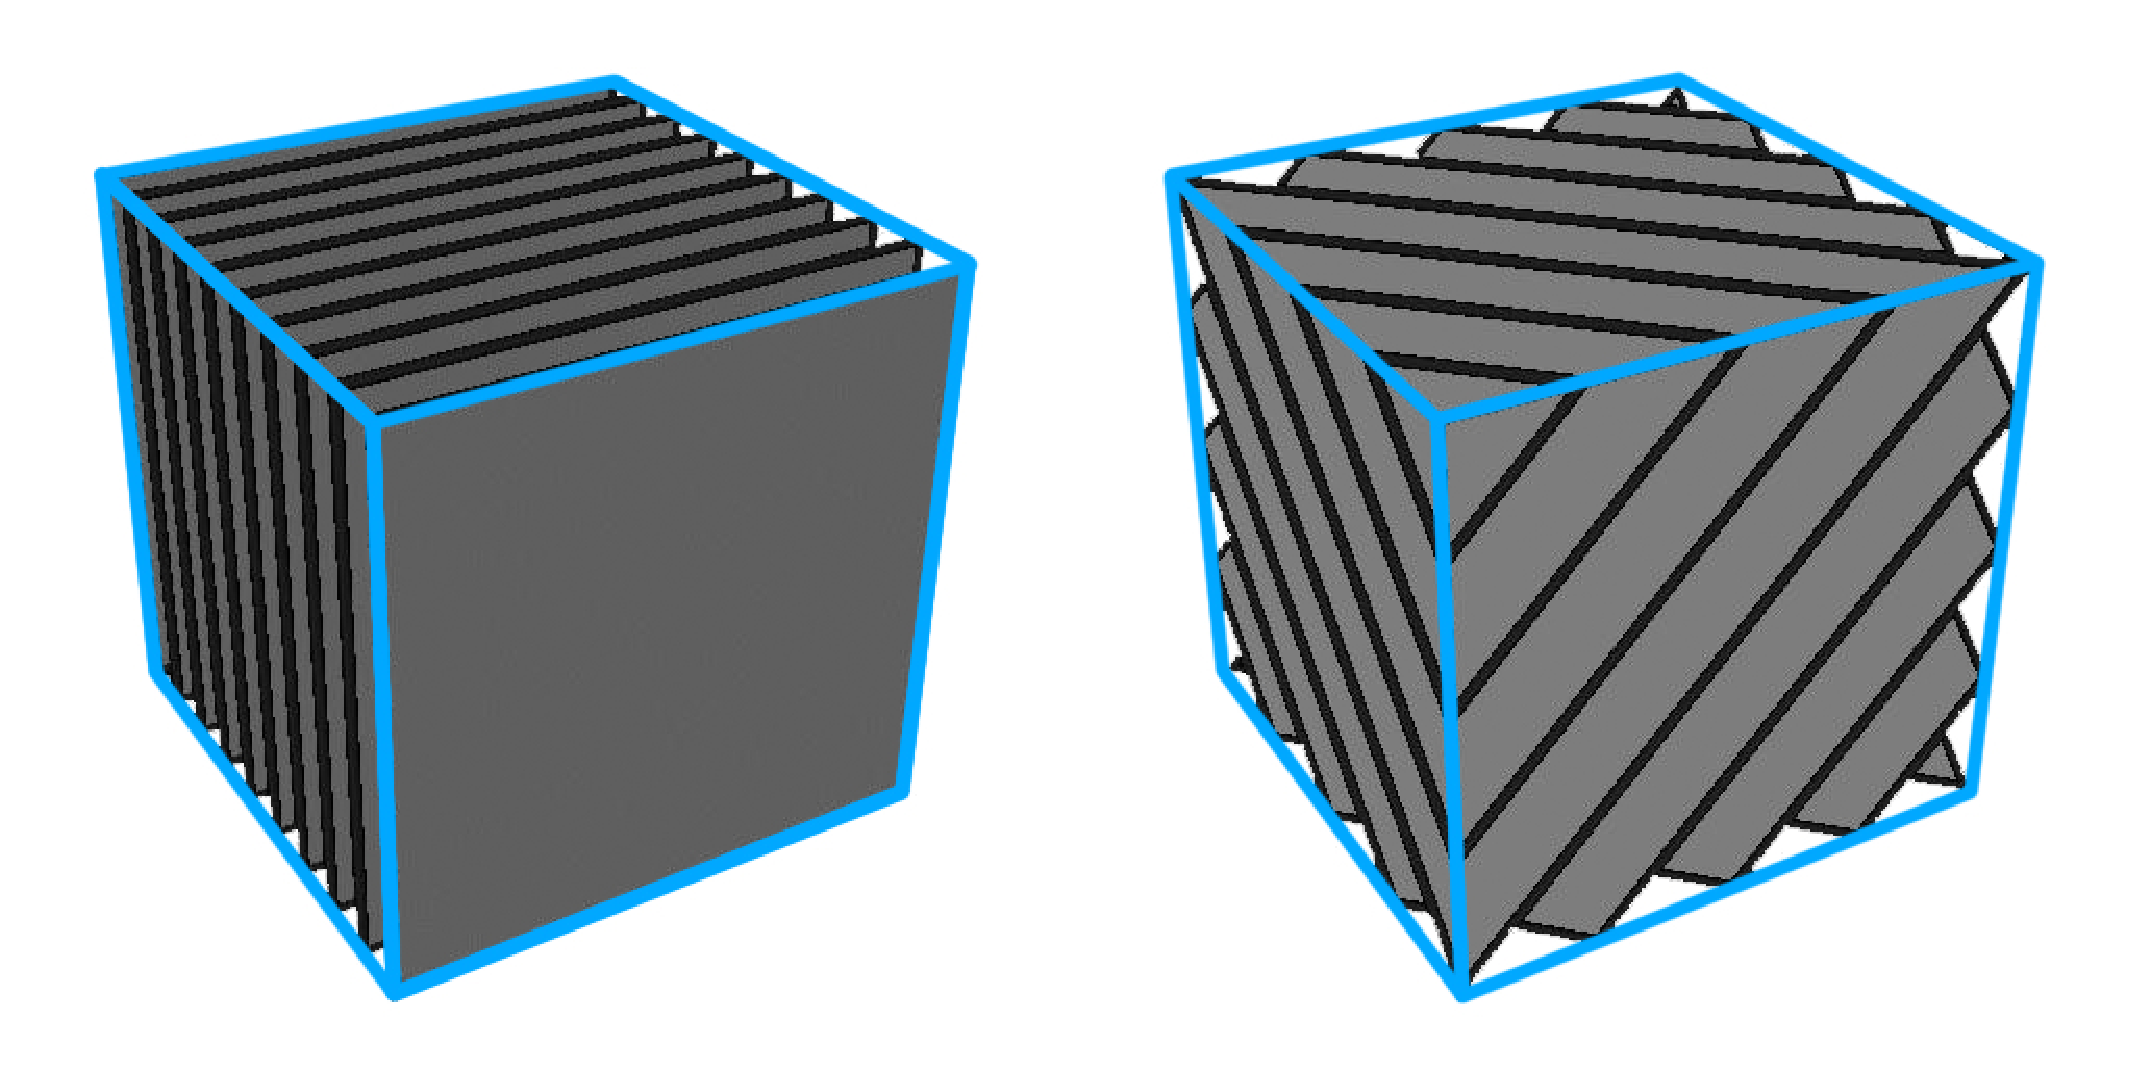
\includegraphics[width=0.7\linewidth]{images/texture_2d3d.pdf}
	\caption{Links: Texturen werden entlang des Volumens ausgerichtet. Rechts: Texturen werden entlang des Blickwinkels ausgerichtet.}
	\label{img:2D3DTex}
	\source{Übernommen von: https://www.evl.uic.edu/aej/524/lecture06.html}
\end{figure}
\FloatBarrier

Liegen die Daten als 3D-Texturen vor, verlaufen die Querschnitte entlang der Sichtachse. Dazu werden sogenannte Proxy-Geometrien erzeugt, Polygone, die einen Querschnitt beschreiben. Auf diesen Proxy-Geometrien wird dann die Textur erstellt, indem die entsprechenden Volumendaten abgefragt werden. Dadurch, dass die Querschnitte an der Sichtachse ausgerichtet sind, ist nur ein Texturstapel notwendig. 


\todo{https://dl.acm.org/citation.cfm?id=329138}

\todo[inline]{implementierung auf der grfikkarte mit 2d texuren nachteil: nur flächen nicht geometrie}
\todo{3d texure based? }	
\todo{Genauer? P}

\begin{figure}[!htb]
	\centering
	%https://www.researchgate.net/figure/Object-aligned-slice-stacks-with-2d-texture-mapping_fig1_226214561
	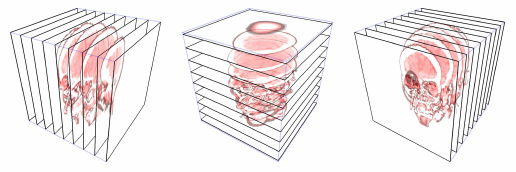
\includegraphics[width=0.7\linewidth]{images/textureStacks.png}
	\caption{Texturen werden als Stapel in der 	XY-, YZ- und XZ-Ebene angeordnet.}
	\label{img:textureBased}
	\source{Übernommen von: \cite{Benassarou05}}
\end{figure}
\FloatBarrier

\subsection{Shear-Warp}

Shear-Warp verfolgt den selben Ansatz wie das Raycasting. Anstatt die Strahlen allerdings von der tatsächlichen Kameraposition aus zu verschießen, werden die Strahlen orthogonal zu den Volumenschichten in das Volumen gefeuert. Auf diese Weise wird die Berechnung der Strahlen und die Komposition der Darstellung deutlich beschleunigt. 
Damit auch bei einem nicht orthogonalen Blickwinkel das Volumen korrekt dargestellt wird, wird vor dem Raycasting eine vom Blickwinkel abhängige Scherung auf die Volumendaten angewandt. In Abbildung \ref{img:shearwarp} ist dargestellt, wie die Scherung die einzelnen Schichten entsprechend des Blickwinkels verschiebt, um einen orthogonalen Einfallswinkel zu simulieren. 
Das durch das Raycasting entstandene Bild wird zunächst in einen Buffer gerendert. Durch die Scherung ist das Bild zu diesem Zeitpunkt noch verzerrt. Deshalb wird es anschließend noch einmal transformiert, sodass eine korrekte Abbildung des Volumens auf die Bildschirmebene projiziert wird. In Abbildung \ref{img:shearwarp} ist zu sehen, wie das gerenderte Bild vor und nach der Transformation aussieht. 
Shear-Warp liefert eine hohe Bildqualität und ist dabei um einiges schneller als Raycastings. 
\todo{begründen warum (GPU-Berechnung, Rasterisierung vs Raytracing)}

\begin{figure}[!htb]
	\centering
	%http://citeseerx.ist.psu.edu/viewdoc/download;jsessionid=97AC0E2CDFD635B2917DF8DF86E99224?doi=10.1.1.548.9543&rep=rep1&type=pdf
	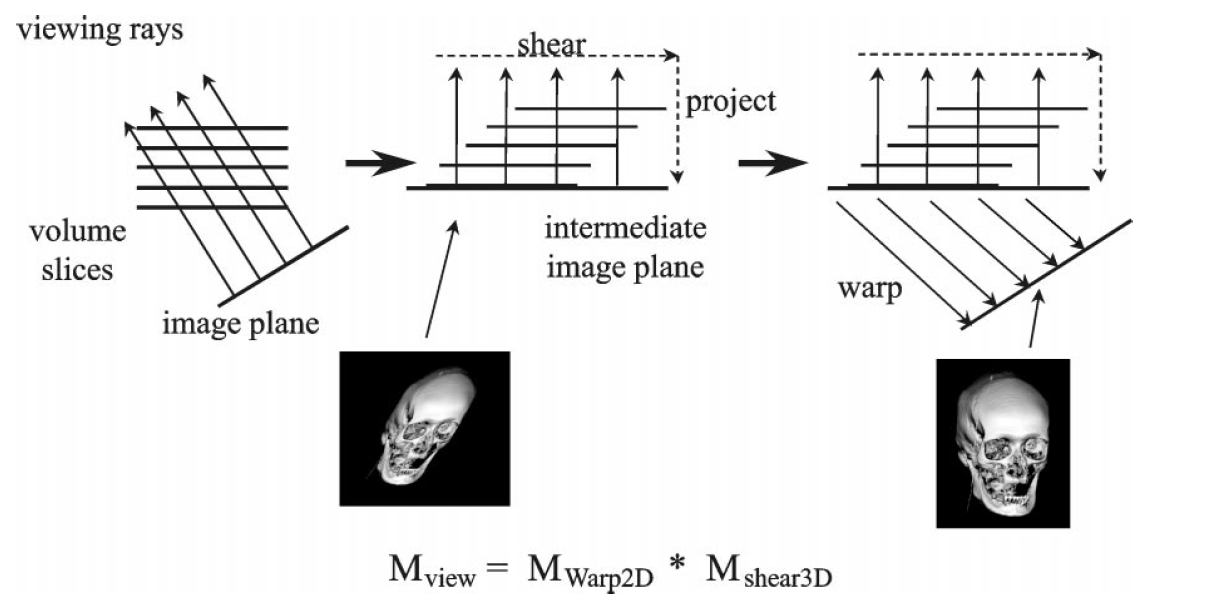
\includegraphics[width=0.7\linewidth]{images/shearwarp.png}
	\caption{Schematische Darstellung des Shear-Warp Verfahrens. Rechts: Ohne Verschiebung würden die Strahlen der Bildebene schräg auf das Volumen treffen. Mitte: Die Schichten des Volumen werden verschoben, sodass die Strahlen orthogonal darauf treffen. Das resultierende Bild ist verzerrt. Rechts: Das verzerrte Bild wird transformiert, um das Volumen korrekt darzustellen.}
	\label{img:shearwarp}
	\source{Übernommen von: \cite{SCHMIDT2000583}}
\end{figure}
\FloatBarrier

%-------------------------------------------------------------
\section{Beispiele für Volume Rendering Implementierungen}
%-------------------------------------------------------------
\label{volumeRenderingImplementierung}

Volume Rendering Techniken werden von verschiedenen Programmen und Arbeiten zur 3D-Visualisierung von MRT-Daten eingesetzt.

Beispiele für Volume Rendering Software sind \textit{MRIcroGL} von \cite{MRIcroGL} und \textit{Voreen}, entwickelt von \cite{voreen}. Die Programme erlauben dabei die Manipulation der Transferfunktion. Ersteres ermöglicht es außerdem bestimmte Bereiche zu markieren und kann durch eigene Skripte erweitert werden.
Die im späteren Abschnitt \ref{radiologieSoftware} genannte MRT-Viewer Software besitzt ebenfalls die Funktionalität die Daten in 3D darzustellen.

Um Volume Rendering spezifisch in \textit{Unity} umzusetzen, existieren die kostenpflichtige \textit{Unity}-Erweiterung \textit{Volume Viewer Pro} von \cite{volumeViewerPro} sowie das \textit{Unity}-Plugin \textit{Unity® Volume Rendering} von \cite{volumeRenderingUnity}. Beide nutzen Volume Raycasting zur Darstellung von 3D-Daten und ermöglichen dem Nutzer das Erstellen einer Transferfunktion über eine Benutzeroberfläche, um das Volumen zu kolorieren. \textit{Volume Viewer Pro} bietet weiterhin das Hervorheben von Bereichen durch ein Overlay, das Laden von NIfTI- und DICOM-Dateien und einige weitere Manipulationsmöglichkeiten. 

Eine der frühesten Arbeiten, die Volume Rendering Techniken vorstellen stammt von \cite{Drebin88}.
\cite{Kruger03} stellen Methoden zur Beschleunigung von Volume Rendering vor.
\cite{Marsalek08} implementieren Volume Raycasting mit CUDA (Compute Unified Device Architecture) von \cite{cuda}, um den Rendering Prozess zu optimieren.
\cite{Kutter08} beschäftigen sich mit der Optimierung von Volume Rendering durch ein AR-HMD\footnote{Head Mounted Display, Erläuterung in Abschnitt \ref{arVr}}. Das Rendering soll interaktiv sein und von den Händen des Nutzers verdeckt werden können.

Vermehrt wird heutzutage Path Tracing oder Monte-Carlo-Raytracing zur Visualisierung von Volumen verwendet. Dabei handelt es sich um ein Verfahren ähnlich dem Raytracing, bei dem zufällig Strahlen in eine Szene geschossen werden, wobei ihr Pfad in der Szene verfolgt wird. Dieser wird durch Reflexion und Absorption, sowie bei Volumen, Streuung bestimmt. Auf diese Weise wird eine globale Beleuchtung der Szene erzeugt. Die Technik wird oft zum Rendern von nicht-körperlichen Volumen, wie Wolken oder Rauch eingesetzt. 
\cite{Fong17} beschreiben Volume Rendering unter Verwendung von Path Tracing, wobei der Fokus auf dessen Einsatz in der Industrie liegt.

%-------------------------------------------------------------
\section{Surface Rendering}		 %
%-------------------------------------------------------------
% Bsp
%Wie in Abschnitt \ref{motivation} beschrieben wurde, bietet eine 3D-Darstellung von MRT-Bildern einige Vorteile gegenüber einer Betrachtung der Daten in 2D. 
% Kann man das belegen?
%Auf Grund dieser Tatsache gab es im Laufe der Zeit verschiedene Ansätze zur Umsetzung einer dreidimensionalen Darstellungsweise. 
%Im Folgenden werden diese erläutert. 

Wie im Abschnitt \ref{volumeData} beschrieben wurde, gibt es neben dem Volume Rendering auch das Surface Rendering. Während ersteres ein Volumen ohne klare Oberfläche abbildet, wird bei Surface Rendering eine Oberfläche aus den Volumendaten erzeugt. Auf diese Weise entsteht ein Mesh des gescannten Objektes.
Im Folgenden wird der Marching Cubes Algorithmus erläutert, ein weit verbreitetes Surface Rendering Verfahren.

% Vor- und Nachteile Tabelle?


\subsection{Marching Cubes}
\label{marchingCubes}
%https://developer.nvidia.com/gpugems/GPUGems3/gpugems3_ch01.html

Das Marching Cubes Verfahren nach \cite{Lorensen87} wird eingesetzt, um eine Polygonenoberfläche zu erzeugen, die ein volumetrisches Objekt visualisiert. 
Der Visualisierung liegen Volumendaten, die in Form eines Skalarfeldes vorliegen zu Grunde.
Die Idee hinter dem Algorithmus ist, dass es zwischen den Voxeln, die innerhalb und außerhalb eines Objektes liegen eine Grenze gibt, die die Oberfläche des Objektes bildet. Diese Grenze gilt es zu finden. 
Die Werte der Voxel, werden dabei als Dichtewerte angesehen. Voxel innerhalb der Grenze haben eine Dichte, die außerhalb eine andere. Demnach kann ein Schwellenwert definiert werden, der die beiden Wertebereiche voneinander trennt.
Um die Grenze zwischen den Voxeln zu ermitteln, werden diese zunächst in Würfel aufgeteilt, woher auch der Name des Verfahrens stammt. Immer vier benachbarte Voxel bilden dabei einen Würfel.  

Die Vorstellung einer Grenze zwischen den Voxeln lässt sich auf die Würfel übertragen. Dabei liegt ein bestimmter Teil der Würfel des Volumens mit allen Eckpunkten innerhalb und ein bestimmter Teil außerhalb des Objektes. Diese Würfel liegen nicht auf der Grenze und alle ihre Eckpunkte haben jeweils ähnliche Werte. Andererseits gibt es Würfel, durch die die Grenze verläuft. Die Eckpunkte dieser Würfel können sich in ihren Werten stark unterscheiden, da jeweils ein Punkt zum Inneren und ein anderer zum Äußeren des Objektes gehören kann. 

Um also die Oberfläche zu erzeugen, die das gesamte Volumen aufteilt, wird jeder Würfel zuerst einzeln betrachtet und es wird ermittelt, ob und wie die Polygonfläche diesen einzelnen Würfel aufteilt.  Die Oberfläche setzt sich dabei aus dreieckigen Polygonen zusammen, sodass auch einzelne Eckpunkte Teil des Objektes sein können.

Die Anzahl an Möglichkeiten einen Würfel aufzuteilen lässt sich errechnen. Für jeden der acht Eckpunkte des Würfels gilt eine von zwei Möglichkeiten: Entweder befindet er sich unter der Oberfläche und damit im Objekt oder eben nicht. Demnach ergeben sich für alle Punkte zusammen $2^8=256$ mögliche Fälle der Aufteilung \cite{aigner07}. Durch den Einbezug von Symmetrie, könnten diese auf 15 verschiedene Möglichkeiten reduziert werden, die in Abbildung \ref{img:marchingCubes} dargestellt sind. Der Fall, dass die Eckpunkte gar nicht getrennt werden ist dabei berücksichtigt. 

\begin{figure}[!htb]
	\centering
	%https://en.wikipedia.org/wiki/Marching_cubes#/media/File:MarchingCubes.svg
	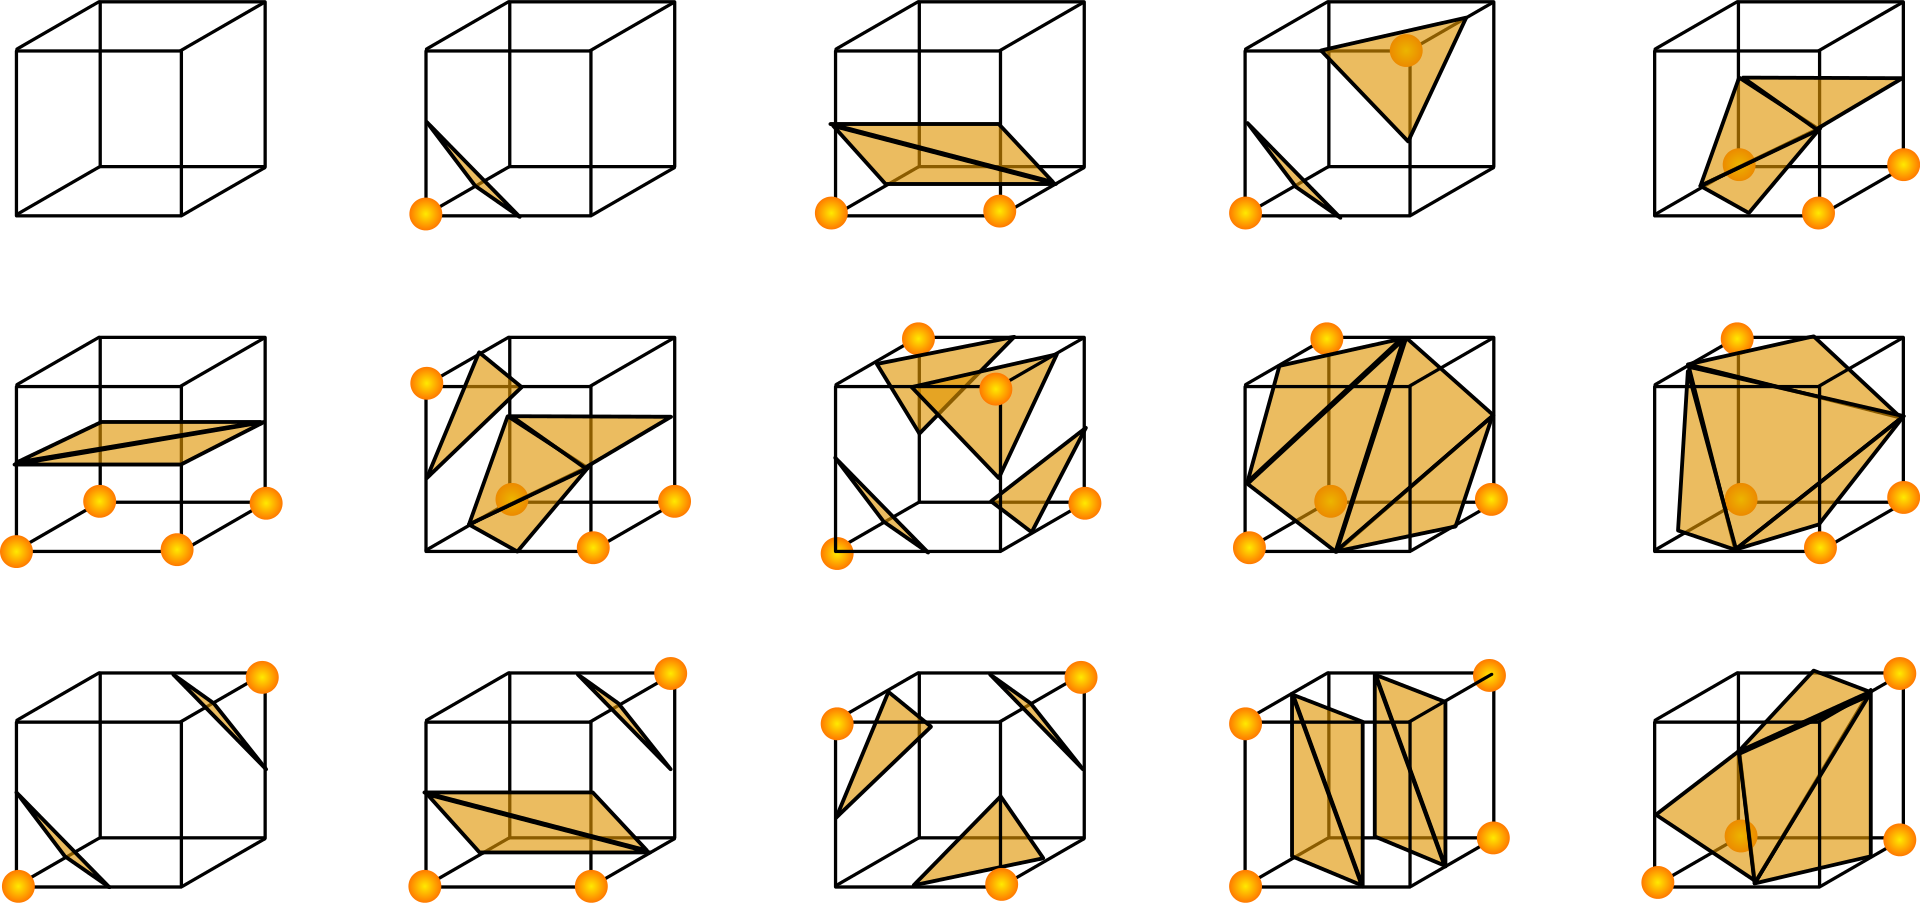
\includegraphics[width=0.7\linewidth]{images/MarchingCubes.png}
	\caption{Die 15 verschiedenen Möglichkeiten, wie eine Polygonfläche einen Würfel in zwei Bereiche teilen kann.}
	\label{img:marchingCubes}
	\source{Übernommen von: https://commons.wikimedia.org/wiki/File:MarchingCubes.svg}
\end{figure}
\FloatBarrier

Bei der Implementierung des Algorithmus werden nun alle 256 Teilungsmöglichkeiten eines Würfels in einer Look-Up-Tabelle gespeichert. Um auszulesen, welcher Fall auf den momentan betrachteten Würfel zutrifft, bedarf es eines Index. 
Der Index ist eine achtstellige Binärzahl. Sie wird ermittelt, indem für jeden der acht Eckpunkte des Würfels geprüft wird, ob er unter dem Schwellenwert liegt, der die Unterscheidung zwischen Innen und Außen definiert oder nicht. Die Ergebnisse der Prüfung, die durch 1 oder 0 repräsentiert werden, werden aneinander gefügt. Nach der Prüfung aller Eckpunkte ist so ein achtstelliger Index entstanden. 

Durch die Verwendung dieses Index und der Tabelle lässt sich so auslesen, wie die Polygone in dem Würfel liegen. Damit ist auch bekannt, auf welchen Würfelkanten sich deren Vertices befinden. Für die Erzeugung einer Oberfläche muss weiterhin die genaue Position des Vertex auf der jeweiligen Kante ermittelt werden. Dies geschieht durch lineare Interpolation zwischen den Werten der Würfeleckpunkte, zwischen denen die betreffende Kante verläuft. 
Auf dieselbe Weise wird für jeden Vertex der Polygone dessen Normale berechnet. Die Normalen der Eckpunkte werden dazu interpoliert.

Nach und nach werden so für jeden Voxelwürfel Polygone berechnet, die in einer Liste gespeichert und schließlich gezeichnet werden.
Der Marching Cubes Algorithmus wird häufig zur prozeduralen Erzeugung von Terrain eingesetzt. In diesem Fall ist es entscheidend, wie die Dichtewerte des Volumens generiert werden. Bei der Visualisierung von medizinischen Daten, wie MRT-Bildern werden die Bilddaten als Eingabewerte genommen.


%https://dl.acm.org/citation.cfm?id=3264776

%https://www.researchgate.net/publication/279205507_A_BRIEF_REVIEW_OF_SURFACE_MESHING_IN_MEDICAL_IMAGES_FOR_BIOMEDICAL_COMPUTING_AND_VISUALIZATION

%-------------------------------------------------------------
\section{Vergleich der Methoden im Überblick}											 %
%-------------------------------------------------------------

\begin{longtable} {p{.2\textwidth}p{.1\textwidth}p{.25\textwidth}p{.35\textwidth}}
 
Methode & Ergebnis & Vorteile & Nachteile \\ 
\toprule 
Volumerisches Raycasting & Rendering  & Sehr gute Bildqualität & Rechenintensiv \\
\midrule 
Shear-Warp & Redering & Sehr schnell& Schlechtere Bildqualität\\
 & & & Benötigt viel Speicher\\
\midrule 
2D-Texture-Based Volume Rendering & Redering & Schnell & Artefakte, wenn aus 45° Winkel gesehen\\
 & &  Wird auch von alten Grafikkarten unterstützt & Abstände zwischen Texturen ist abhängig von Blickrichtung \\
 & & benötigt nur bilinieare Interpolation &  Artefakte bei Rotation\\ 
\midrule 
3D-Texture-Based Volume Rendering & Rendering & keine Artefakte durch Blickwinkel & langsamer durch trilineare Interpolation \\
 & &  Abstand zwischen Texturen konstant & Grafikkarte braucht 3D Texturen Unterstützung\\ 
 & & & Artefakte bei Rotation\\
\midrule 
Marching Cubes & 3D-Mesh &  &\\ 
\bottomrule
\caption{\label{tab:volumeRenderingVergleich}Vergleich von Methoden zur 3D Darstellung von Volumendaten}
\end{longtable}

\todo{Tabelle zu Text: Vergleich zwische geschwindigkeit, bildqualität und implementierungsaufwand}
%-------------------------------------------------------------
\section{AR und VR}		
\label{arVr}							 %
%-------------------------------------------------------------

mARt ist als AR-Anwendung konzipiert. Eine Umsetzung in VR wäre aber ebenso denkbar und dient, wie in Abschnitt \ref{device} beschrieben wird als Alternative.
Deshalb werden die beiden Technologien an dieser Stelle vorgestellt, um ein Verständnis für die Begriffe, ihre Ausprägungsformen und Funktionsweisen zu schaffen.

\subsection{Augmented Reality}

Der Begriff der Augemented Reality (AR), also Erweiterte Realität, beschreibt die Idee, dass die physisch vorhandene Welt, die einen Nutzer umgibt, mit zusätzlichen digitalen Inhalten angereichert wird. Dies geschieht z.B. indem wahrgenommene Gegenstände von virtuell erzeugten Objekten überlagert werden. 
Laut \cite{azuma97} zeichnet sich eine AR-Anwendung durch folgende Eigenschaften aus:

\begin{itemize}
\item Kombiniert reale und virtuelle Realität
\item Ist in Echtzeit interaktiv
\item 3D-Objekte existieren in dreidimensionaler Realität
\end{itemize}

AR und VR verbindet eine ähnliche Geschichte. Die frühesten VR-Systeme waren nach heutiger Definition AR-Systeme. \todo{Referenz?}
%Geshcihte?
Viele AR-HMDs funktionieren mit Stereoskopie (s. Abschnitt \ref{vr}). Die eben genannten Definition lässt allerdings auch andere Systeme zu. 
Beispielsweise kann eine AR-Anwendung mit oder ohne einen Bildschirm konzipiert werden, der die Augmentierung darstellt. Im letzteren Fall werden dann meist Beamer o.Ä. verwendet, um die Objekte in die reale Welt zu projizieren. 
Wie aus den in Abschnitt \ref{relatedAR} vorgestellten Arbeiten hervorgeht, verwendet die Mehrzahl von AR-Software allerdings Bildschirme. 
Aber auch hier gibt es verschiedene Lösungsansätze. Dies betrifft zum einen die Positionierung des Bildschirms. Dieser kann direkt vor dem Auge des Nutzers, in der Welt oder in einem tragbaren Endgerät platziert werden.
Weiterhin können Bildschirme durchsichtig oder undurchsichtig sein. Handelt es sich um einen durchsichtigen Bildschirm, wird darauf nur die Augmentierung dargestellt. Der Vorteil hierbei ist, dass der Nutzer seine Umgebung größtenteils unverfälscht wahrnehmen kann. Damit ist aber gleichzeitig der Kontrast zu den nicht unbedingt realitätsnahen 3D-Objekten größer.
Bei undurchsichtigen Bildschirmen nimmt eine Kamera die Umgebung auf und gibt sie augmentiert auf dem Bildschirm aus. Diese Technik wird z.B. verwendet wenn AR-Anwendungen für Smartphones oder Tablets entwickelt werden. In Abbildung \ref{img:ARMarker} ist dargestellt, wie eine solche Anwendung auf einem Smartphone aussieht.

\begin{figure}[!htb]
	\centering
	%https://commons.wikimedia.org/wiki/File:App_iSkull,_an_augmented_human_skull.jpg
	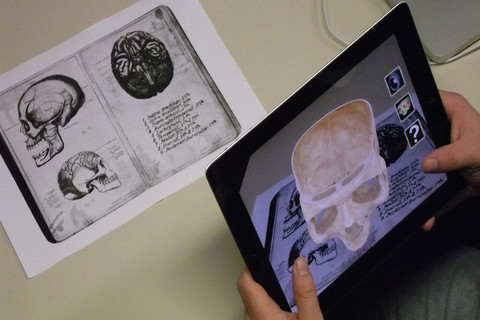
\includegraphics[width=0.5\linewidth]{images/App_iSkull,_an_augmented_human_skull.jpg}
	\caption{Eine tabletbasierte AR-Anwendung, die auf einem Marker des 3D-Modell  eines Schädels projiziert.}
	\label{img:ARMarker}
	\source{Übernommen von: https://commons.wikimedia.org/wiki/File:App\_iSkull,\_an\_augmented\_human\_skull.jpg}
\end{figure}
\FloatBarrier

Alle Techniken haben gemeinsam, dass eine Kamera Teil des Systems ist, die die Umgebung des Nutzers aufnimmt. Dadurch werden Tiefen- und Bildinformationen gesammelt. Durch die Auswertung dieser und anderer Informationen, wie z.B. GPS- oder Wlan-Daten, können 3D-Objekte korrekt mit der Umgebung in Beziehung gesetzt werden. So ist es möglich ein virtuelles Objekt auf oder hinter ein reales zu stellen. Durch ein möglichst umfassendes Verständnis des umgebenden Raumes ist es auch möglich, dass die Elemente der erweiterten Realität in der realen Welt an der richtigen Stelle platziert werden und dort auch bleiben.
Alternativ dazu können am gewünschten Ort Markierungen gesetzt werden, die das System erkennt und somit genau dort das 3D-Modell darstellen kann. Solche Marker können unterschiedlich aussehen. Oft werden komplexe schwarz-weiße Muster dafür verwendet, weil diese gut zu identifizieren und schwer zu verwechseln sind. In Abbildung \ref{img:ARMarker} ist ein 3D-Objekt zu sehen, dass auf einem Marker platziert wurde. 

Zurzeit gibt es verschiedene AR-Systeme auf dem Markt, die sich teilweise in ihrer Funktionsweise unterscheiden. Relevant sind dabei vor allem Smartdevices sowie binokulare Head Mounted Displays (HMDs) die eigens für AR-Anwendungen konzipiert sind.

Smartphones oder Tablets können, wie bereits erwähnt als Fenster in die erweiterte Realität dienen. Das Gerät benötigt dazu lediglich eine Kamera. Es gibt verschiedene SDKs und Frameworks zur Entwicklung von AR-Apps. Dazu gehören unter anderem \textit{ARKit} von \cite{arKit}, \textit{ARCore} von \cite{ARCore} und \textit{Vuforia} von \cite{vuforia}.

Zu den binokularen HMDs zählen HMDs, die vor jedem Auge des Nutzers einen Bildschirm platzieren und so stereoskopisch dreidimensionale Inhalte simulieren. Im AR-Bereich sind dabei die \textit{HoloLens} von \cite{hololens} sowie die \textit{Magic Leap One} von \cite{magicLeap} nennenswerte Vertreter der Technologie. Beide Geräte haben durchsichtige Bildschirme und können unabhängig von einem Computer verwendet werden. 
Der Bildschirm nimmt dabei allerdings nur einen Teil des Blickfeldes des Nutzers ein. Bei der \textit{HoloLens} beträgt das Sichtfeld 30°x17,5° \cite{hololensFOV}. Dies führt zu dem Effekt, dass der Nutzer die augmentierten Inhalte wie durch ein Fenster sieht, sodass sie häufig teilweise abgeschnitten sind. Auf diese Problematik wird im Kapitel \ref{ergebnisse} eingegangen. 

An dieser Stelle sollen auch VR-Geräte, wie die \textit{HTC Vive Pro} (Vive Pro) von \cite{vivePro} genannt werden, die durch ihre eingebaute Kamera auch die Umgebung auf ihren Bildschirmen darstellen kann. Diese kann dabei auch mit virtuellen Inhalten angereicherts werden. 
mARt ist wie im Kapitel \ref{konzept} beschrieben für ein HMD konzipiert.

%Ebenfalls als HMD zu bezeichnen ist die \textit{Google Glass} von \cite{googleGlass}. Dabei handelt es sich um ein Brillengestell, dass vor einem der Augen des Nutzers einen durchsichtigen Bildschirm fixiert, auf dem digitale Inhalte dargestellt werden können. Google Glass wird momentan allerdings nur noch von Firmen verwendet.

\subsection{Virtual Reality}
\label{vr}

Im Gegensatz zu AR wird der Nutzer bei Virtual Reality (VR) von seiner realen Umgebung abgeschnitten und in eine simulierte versetzt, mit der er in Echtzeit interagieren kann. Dabei wird in der Regel eine möglichst hohe Immersion angestrebt. 
Im Kontext von VR bezeichnet Immersion den Effekt, dass ein Nutzer dermaßen in die simulierte Welt, die ihn umgibt eintaucht, dass sich diese für ihn real anfühlt und Interaktionen mit ihr natürlich werden (vgl. \cite{Witmer98}). Wie immersiv eine Anwendung ist, hängt dabei von der Anwendung selbst ab, sowie auch von dem verwendeten VR-System. 

Im Laufe der Zeit wurden verschiedene Systeme entwickelt, die ein möglichst immersives Erlebnis erschaffen sollten. 
Bereits in den 50er Jahren wurde versucht den Nutzer in das Geschehen eines Films zu versetzten, indem er von seiner realen Umgebung isoliert und seine Wahrnehmung so auf bestimmte Reize gebündelt wurde, z.B. durch das \textit{Sensorama} \cite{sensorama}. % Referenz Sensorama
In den 1960ern wurden von \cite{Sutherland68} die erste Versionen eines HMD entwickelt. %Referenz Sword of Dmaocles -> Eigentlich AR
Um den Eindruck von Dreidimensionalität zu erzeugen, wird für binokulare HMDs in den meisten Fällen das Prinzip der Stereoskopie verwendet. Hierzu werden jeweils dem linken und rechten Auge des Nutzers zwei Bilder des selben Objektes aus leicht unterschiedlichen Blickwinkeln  gezeigt. Da die Augen beim normalen Sehen ein Objekt tatsächlich aus zwei verschiedenen Winkeln wahrnehmen, werden die Bilder im Gehirn zusammengefügt, sodass der Eindruck von Tiefe entsteht. Die Bilder werden dabei auf zwei Bildschirmen direkt vor dem Auge angezeigt, vor die eine Linse gesetzt wird, um die Illusion zu erzeugen, dass das Gezeigte weiter entfernt ist als in der Realität und es dem Auge zu ermöglichen die Bilder trotz der Nähe zu fokussieren.

Der Blickwinkel auf ein Objekt hängt dabei von der Kopfposition des Nutzers ab. Um diesem die Möglichkeit zu geben, den Kopf zu bewegen und damit den Eindruck eines 3D-Objektes zu verstärken, wird die Position des Kopfes verfolgt. Auf diese Weise können die stereoskopischen Bilder an den Blickwinkel des Nutzers angepasst werden. Dieser erhält somit das Gefühl, er könne um das dargestellte Objekt herumgehen. 

Die Bewegungsfreiheit der Nutzers war allerdings durch die damalige Technik eingeschränkt, denn das System, mit dem das HMD verbunden war, war zu schwer, um es zu tragen und deshalb fest installiert. 
In den 90er Jahren gab es deshalb Entwicklungen in eine andere Richtung. Anstatt die virtuelle Realität nur direkt vor den Augen des Nutzers darzustellen, sollte diese um ihn herum erzeugt werden. Dazu wird der Nutzer in einem abgeschlossenen Raum platziert, an dessen Wände und Boden die Umgebung des jeweiligen Szenarios projiziert wurde. Die Immersion des Erlebnisses kann gesteigert werden, indem z.B. 3D-Brillen eingesetzt werden. Sogenannte CAVE-Systeme (Cave Automatic Virtual Environment) kommen auch heute noch zum Einsatz. Da sie allerdings sehr unhandlich und in ihrer Umsetzung kostspielig sind, eignen sie sich nicht als Massenprodukt oder für private Nutzung.
\todo{Referenz
}
Obwohl die Simulation einer virtuellen Realität oft auf die Täuschung visueller Wahrnehmung fokussiert ist, werden in vielen Systemen auch andere Sinne angesprochen, um das Erlebnis immersiver zu gestalten. Dies gilt vor allem für das Gehör. Dem Nutzer werden dabei über Lautsprecher oder Kopfhörer zur Erfahrung passende Geräusche vorgespielt.
Eine größere Herausforderung stellt die Imitation von haptischen Reizen dar. Hierzu gibt es verschiedene Ansätze. Einer der einfacheren ist es dem Nutzer bei virtuellen Berührungen Vibrationen auszusetzen, z.B. über Eingabemedien in seinen Händen. Es gibt allerdings mehrere Konzepte, die haptische Impulse realistischer simulieren sollen, beispielsweise durch Handschuhe aus speziellem Material. %Referenz 
Durch die Verwendung eines Laufbands, das auf die Laufbewegung des Nutzers reagiert soll die Bewegungsfreiheit innerhalb der Simulation erweitert werden. Omnidirektionale Laufbänder können sowohl zusammen mit HMDs als auch CAVEs eingesetzt werden.
Über den Verlauf der Entwicklung von VR-Systemen wurde außerdem des Öfteren versucht Gerüche zu simulieren.  \todo{Referenz??}
Auf die Möglichkeiten der Nutzerinteraktion in VR-Systemen wird im Abschnitt \ref{VRInteraktion} genauer eingegangen.

Heutzutage bestehen die meistgenutzten VR-Systeme aus einem HMD, welches über eine Kamera verfügt, Eingabemedien (z.B. Controllern), einem Trackingsystem, das die Position der ersten beiden Komponenten verfolgt und einem Computer, der die Komponenten miteinander verknüpft und auf dem die VR-Anwendung läuft. 
In Abbildung \ref{img:vive} ist ein HMD und die dazugehörigen Controller während der Nutzung abgebildet.

\begin{figure}[!htb]
	\centering
	%https://sco.wikipedia.org/wiki/Virtual_reality#/media/File:Reality_check_ESA384313.jpg
	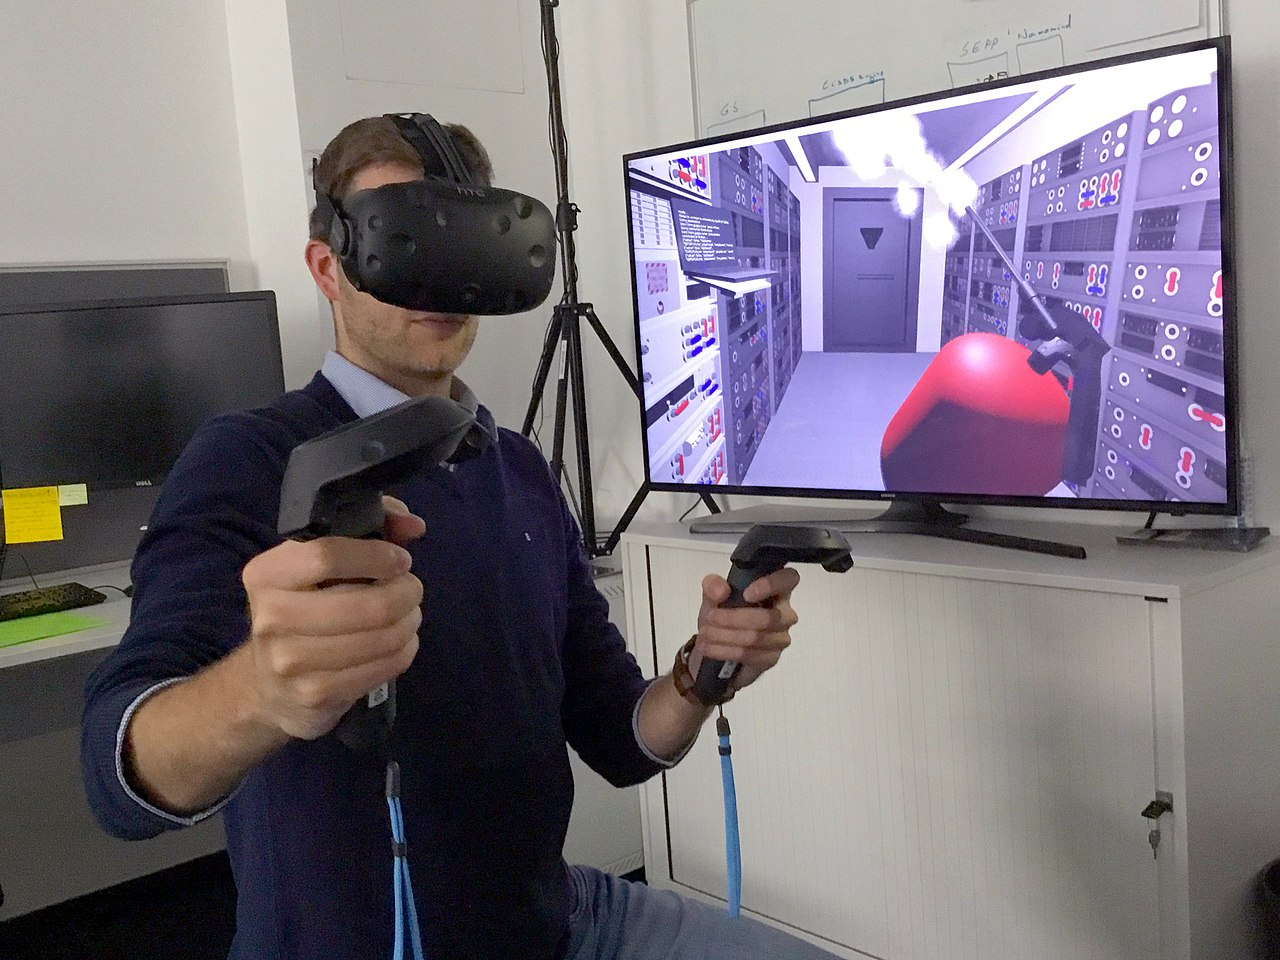
\includegraphics[width=0.5\linewidth]{images/vive.jpg}
	\caption{Ein Nutzer trägt das HMD der \textit{Vive} und bedient dessen Controller.}
	\label{img:vive}
	\source{Übernommen von: https://sco.wikipedia.org/wiki/Virtual\_reality\#/media/File:Reality\_check\_ESA384313.jpg}
\end{figure}
\FloatBarrier

%-------------------------------------------------------------
\section{Verarbeitung von MRT-Daten in der Neurologie}						 %
%-------------------------------------------------------------
 
\subsection{Diagnose von Schlaganf\"allen durch bildgebende Verfahren}
\label{schalganfaelleMRT}

Wie bereits in Abschnitt \ref{motivation} erläutert wurde, besteht der Nutzen eines MRTs darin, dass der behandelnde Arzt einen Einblick in die betreffenden Organe (hier das Gehirn) erhält. Dazu studiert er die einzelnen Schichten des Gehirns und sucht nach Anomalien.
Im Folgenden wird erläutert, wie ein Schlaganfall durch bildgebende Verfahren diagnostiziert wird.
Der vom Schlaganfall betroffene Bereich des Gehirns wird anschließend vom Arzt auf jeder einzelnen Schicht markiert.

Laut der \cite{schlaganfall} bezeichnet ein Schlaganfall eine plötzlich auftretende Störung der Gehirnfunktionen durch eine mangelhafte Durchblutung von Gehirnpartien. Die Nerven im Gehirn werden dabei nicht mit genügend Sauerstoff versorgt, was irgendwann zu Beschädigungen des Gehirns führen kann.

Die Diagnose eines Schlaganfalls erfolgt durch bildgebende Verfahren, wie MRT- oder CT-Scans. Anhand der Bilder kann ein Neurologe erkennen, um welche Art von Schlaganfall es sich handelt und ob dieser durch eine Hirnblutung oder einen Gefäßverschluss ausgelöst wurde. 

Die Besonderheiten in der Untersuchung von CT- und MRT-Bildern wird von \cite{schlaganfallBilder} beschrieben.
Oft wird dabei zuerst ein CT-Scan durchgeführt, da dieser schneller Ergebnisse liefert und meist verfügbarer ist, auch wenn die Qualität der Ergebnisse geringer ist als bei einem MRT. 
Auf einem CT-Scan können anhand der Form und Struktur des Gehirns Schwellungen entdeckt werden, die von einer Gefäßverstopfung herrühren können. Besonders gut auf CT-Bildern zu erkennen sind Hirnblutungen, da das austretende Blut als heller Bereich auf den Bildern dargestellt wird. 

Eine MRT liefert nicht nur genauere Bilder sondern kann unzureichend durchblutete Bereiche früher nach dem Eintreten der Schlaganfallsymptome verlässlich sichtbar machen, als es bei einer CT der Fall ist.
Der minderdurchblutete Bereich des Gehirns wird auf MRT-Bildern heller dargestellt als der Rest des Gewebes. Er wird von Neurologen markiert, um die Ausmaße und Lage des Schadens zu bestimmen und soll in mARt zusammen mit den MRT-Daten angezeigt werden können.

Nach der Diagnose wird versucht, das Blutgerinnsel durch Verabreichung von Medikamenten aufzulösen oder es mechanisch zu entfernen. Bei einer Hirnblutung kann ein operativer Eingriff nötig sein.
\cite{schlaganfallBehandlung}

\subsection{Visualisierungssoftware in der Neurologie}
\label{radiologieSoftware}
% https://www.dicomlibrary.com/meddream/md5/index.html?study=1.2.826.0.1.3680043.8.1055.1.20111102150758591.92402465.76095170
%Use Cases
%Bsp
Um eine Diagnose stellen zu können, muss der Arzt die MRT-Bilder eines Patienten genau studieren. Diese Untersuchung der Daten wird digital durchgeführt. Um dem Arzt einen Einblick in den Datensatz zu geben, gibt es spezielle Anzeigeprogramme, die diesen darstellen können und weiterhin Manipulationsmöglichkeiten bieten. 
  
Wie bereits beschrieben, liegen die MRT-Bilder meist im DICOM- oder NIfTI-Datenformat vor. Um die Dateien öffnen zu können, bedarf es deshalb bestimmter Software. Es stehen viele verschiedene Programme zur Darstellung von MRT-Bildern zur Verfügung und die Auswahl eines Programms hängt meist von der persönlichen Präferenz des Arztes ab. 
In Krankenhäusern besteht allerdings in der Regel die Situation, dass die Bilder in einem Picture Archiving and Communication System (PACS) gespeichert werden. Dabei handelt es sich um einen Server, der unter anderem medizinische Bilddaten zentral speichert. Die Bilder werden von bildgebenden Verfahren aus z.B. der Radiologie direkt im PACS gespeichert. Von dort aus kann entweder mit speziellen Arbeitsplatzrechnern oder auch mit privaten Computern über den Browser auf die Bilder zugegriffen werden. Dies geschieht dann meistens durch einen entsprechenden Viewer, der in das PACS integriert ist. Die Speicherung und Verteilung von medizinischen Bilddaten ist oft durch den DICOM-Standard geregelt, der im Abschnitt \ref{datenformate} beschrieben wurde.

Die meisten Viewer-Programme für MRT-Bilder, unabhängig davon, ob es sich um PACS-Viewer handelt oder nicht, ähneln sich stark in den Funktionen die sie anbieten und in ihrem Aufbau.

Meist können in mehreren Fenstern verschiedene Ansichten des gleichen oder unterschiedlicher Datensätze geöffnet werden. Jedes Fenster stellt dabei eine Sichtebene dar, die gleichzeitig den Querschnitt durch das Gehirn bildet. Die verschiedenen Sichtebenen können in den anderen Ansichten farblich kodiert eingezeichnet werden, damit der Arzt ein besseres Bild davon bekommt welchen Teil des Gehirns er gerade betrachtet.
Üblicherweise werden drei verschiedene Blickwinkel dargestellt, die an den X-, Y- und Z-Achsen ausgerichtet sind. Die Sichtebenen verlaufen dabei orthogonal zur Blickachse. Die Ebenen können entlang der Achsen verschoben werden. Auf diese Weise scrollt der Neurologe durch die verschiedenen Schichten des Gehirns. 
Bei den drei Ebenen handelt es sich um die Frontal- oder Coronalebene, die das Gehirn in vorne und hinten teilt, die Sagittalebene, die zwischen links und rechts verläuft und die Transversalebene, die eine Teilung zwischen oben und unten bewirkt.  
Bei dieser Zusammensetzung von Ebenen wird manchmal noch eine vierte Ansicht ergänzt, auf der entweder die Sagittalebene von der anderen Seite abgebildet ist oder durch das Ineinanderschieben der gerade angezeigten Schichten eine annähernd dreidimensionale Darstellung simuliert wird. 
In Abbildung \ref{img:mrtSoftware} ist die Oberfläche de \textit{OsiriX DICOM Viewers} zu sehen, die beispielhaft die Ansichten zeigt.

\begin{figure}[!htb]
	\centering
	%https://www.macupdate.com/app/mac/14362/osirix
	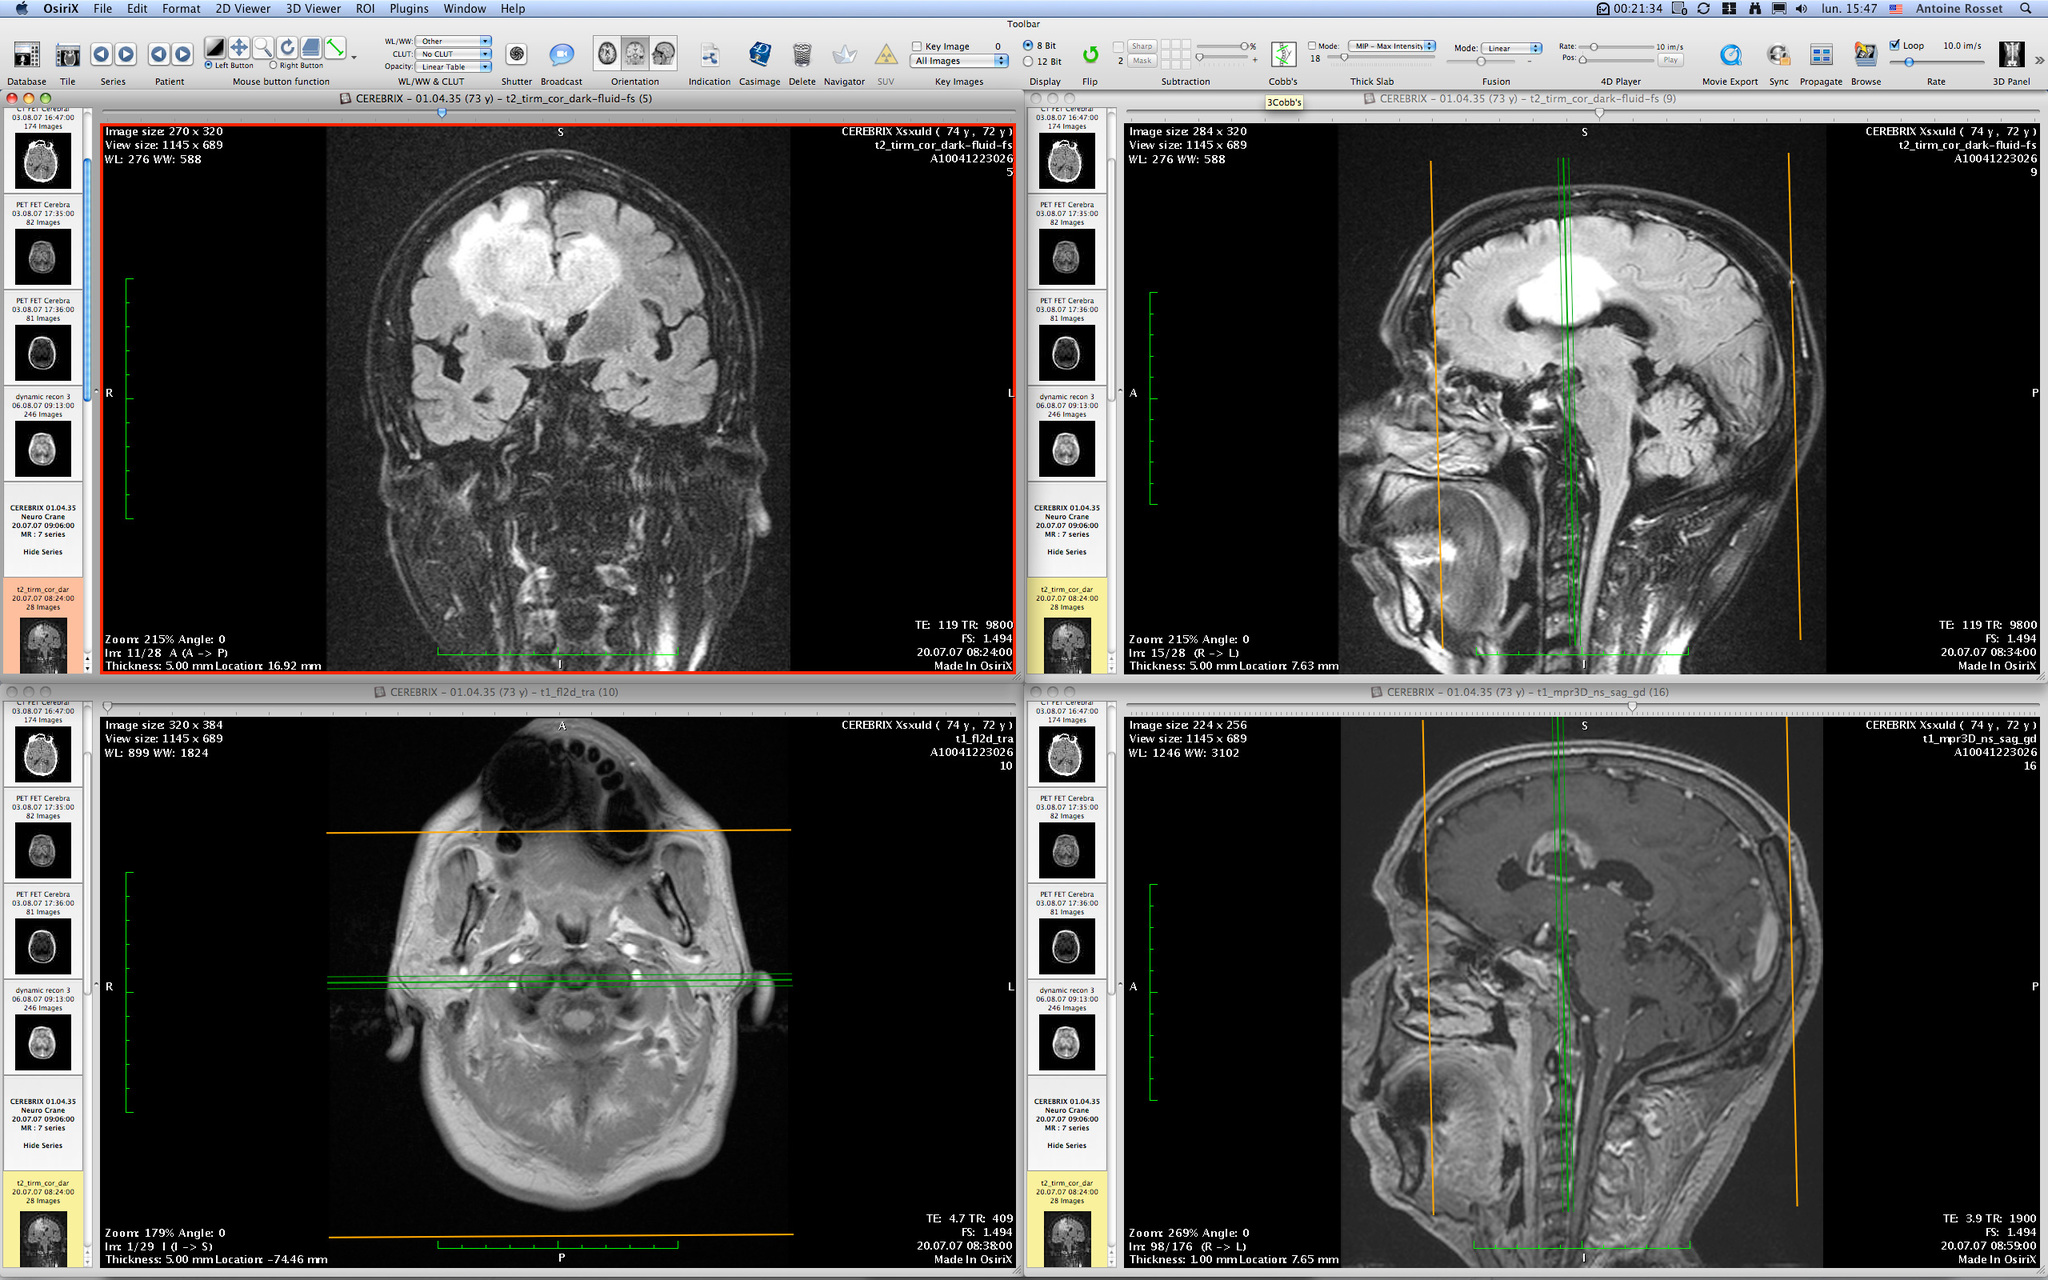
\includegraphics[width=0.7\linewidth]{images/osirix.jpg}
	\caption{Die Benutzeroberfläche des \textit{OsiriX DICOM Viewers}. Der Scan eines Kopfes wird aus den drei klassischen Perspektiven angezeigt. Die Position der ausgewählten Sichtebene ist in den übrigen Fenstern farbig eingezeichnet.}
	\label{img:mrtSoftware}
	\source{Übernommen von: https://www.macupdate.com/app/mac/14362/osirix}
\end{figure}
\FloatBarrier

Die Benutzeroberfläche bietet auch einige Interaktionen. Die wichtigsten sind dabei die, die es dem Arzt ermöglichen ein möglichst eindeutiges Verständnis vom Inneren des Gehirns zu erhalten.  Dazu zählen:

\begin{description}
\item [Scrollen durch die einzelnen Bildschichten]\hfill \\
Dies geschieht in der Regel durch die Auswahl einer der Ansichten und die Betätigung des Mausrads. 
\item [Einstellen von Kontrast und Helligkeit]\hfill \\
Dadurch können schlecht sichtbare Strukturen erkennbarer gemacht werden. Das Werkzeug dazu muss in der Taskleiste ausgewählt werden. In einem separaten Fenster können die Werte dann angepasst werden. 
\item [Heranzoomen]\hfill \\
Bestimmte Bereiche eines Bildes können vergrößert werden, um sie besser beurteilen zu können.
\item [Verschieben des Bildausschnitts]\hfill \\
Um über ein vergrößertes Bild zu navigieren, kann der Nutzer dieses anklicken und in eine Richtung ziehen. Dies ermöglicht es andere Bildteile zu untersuchen, ohne zuerst das Bild verkleinern zu müssen.
\end{description}

Obwohl über die Taskleiste oft noch weitere Optionen zur Verfügung stehen sind diese nicht essenziell zur Untersuchung der Bilder und werden meistens nicht oder nur in geringem Umfang genutzt, wie aus den Interviews mit einem Neurologen hervorging.

Es gibt eine Vielzahl von Viewern dieser Art zum Öffnen oder zur Verarbeitung von MRT-Bildern. Viele davon stehen kostenlos im Internet zur Verfügung. 
Zu den wahrscheinlich meist verbreitetsten gehören \textit{OsiriX} von \cite{osirix} und \textit{Horos} von \cite{horos}, für das Betriebsystem \textit{macOS} von \cite{macOs}. \cite{radiocafe} stellt außerdem folgende Viewer zum Gebrauch im radiologischen Kontext für andere Betriebssysteme vor: Das kompakte und schnelle Viewerprogramm \textit{RadiAnt} von \cite{radiant}. Weiterhin \textit{Stratovan Pro Surgical 3D} von \cite{prosurgical}, was sich an Chirurgen richtet und \textit{Navegatium DICOM Viewer} von \cite{navegatium}, ein Programm, dass auch als App und somit auch für Tabletts zur Verfügung steht.
Alle der genannten Viewer besitzen die Funktion aus MRT-Datensätzen auch Volumendarstellungen zu erzeugen.

%-------------------------------------------------------------
\section{Interaktion in AR/VR}	
\label{VRInteraktion}							 %
%-------------------------------------------------------------

Nachdem die Interaktionsmöglichkeiten bisher bestehender Visualisierungssoftware beschrieben wurden, sollen an dieser Stelle Optionen vorgestellt werden, wie Interaktionen in AR und VR stattfinden können. 

\subsection{Systeminterne Nutzereingaben}

VR- und AR-Systeme, die momentan auf dem Markt verfügbar sind, besitzen in der Regel  eine oder mehrere Formen der Eingabe, um mit dem System zu interagieren. Da mARt als AR-Anwendung konzipiert ist, werden die verschiedenen Mittel zur Eingabe an dieser Stelle vorgestellt.
Die Eingabemöglichkeiten sind dabei teilweise von der Art des Systems abhängig. 
Beispielsweise kann für Smartphone-Apps der Touchbildschirm des Gerätes für die Nutzereingabe genutzt werden. 

Theoretisch kann jedes System mit jedem Eingabemedium verknüpft werden. Dies ist allerdings für Nutzer und Entwickler mit entsprechendem Aufwand verbunden. Die Techniken, die von den derzeit erhältlichen AR und VR Systemen verwendet werden, werden im Folgenden vorgestellt.
%IMMERSION

\paragraph{Controller}
Zum einen gibt es Controller, die mit dem System zusammen hergestellt werden und die der Nutzer während der Verwendung des Systems in der Hand hält. Im Fall von VR-Systemen sind meistens zwei Controller vorhanden, einer für jede Hand. Diese sind jeweils mit einer Anzahl an Knöpfen oder auch Touchpads versehen, die der Nutzer bedienen kann. Im Aussehen sind sich Controller dieser Art recht ähnlich. In Abbildung \ref{img:VRController} ist der Controller des \textit{HTC Vive} Systems (\textit{Vive}) von \cite{vive} zusehen.
\todo{Bild einfügen}
Allerdings existieren auch Systeme für deren Bedienung nur ein Controller vorgesehen ist. Ein VR-Beispiel ist die \textit{Oculus Go} von \cite{oculus}, ein eigenständiges System für grafisch weniger anspruchsvolle Anwendungen. 
Auch AR-Systeme, wie die \textit{Magic Leap} von \cite{magicLeap} oder die \textit{HoloLens} besitzen nur einen Controller. Diese haben im Vergleich zu den zuerst genannten VR-Controllern deutlich weniger Eingabemöglichkeiten. Im Falle der \textit{Hololens} handelt es sich um einen flachen Controller, den sich der Nutzer an den Finger steckt. Indem er Druck ausübt, kann er klicken. Daneben wird nur die Position und Rotation des Clickers verfolgt, durch die der Nutzer mit dem System interagieren kann. Das Gerät stellt damit eine von zwei möglichen handgesteuerten Eingabemethoden dar. 

\paragraph{Gesten}
Die andere ist die Steuerung über Gesten, die vor allem AR-Systeme verwenden.
Die in den Systemen verbaute Kamera erfasst dabei die Hände des Nutzers in ihrem Blickfeld und erkennt bestimmte Handgesten, auf die dann reagiert wird. 
Die \textit{HoloLens} kann zum aktuellen Zeitpunkt zwei Hauptgesten erkennen, \textit{Bloom} und \textit{Air tap}, sowie die Bewegung der Hand. Durch die Verbindung von beidem können beispielsweise Objekte verschoben werden. In Abbildung \ref{img:hololensGestures} ist dargestellt, wie die Hololens-Gesten ausgeführt werden. 
Die derzeit angekündigte \textit{HoloLens 2} verfügt dagegen über eine Hand-Tracking-Funktionalität, die jede Bewegung der Hände, wie z.B. das Greifen von Objekten erkennt (vgl. \cite{hololens2}). 
Die \textit{Magic Leap} erkennt dagegen acht verschiedene Handgesten, die in \ref{img:magicGestures} abgebildet sind. 


\begin{figure}[!htb]
	\centering
	%https://www.researchgate.net/figure/The-common-air-tap-gesture-used-in-the-HoloLens-application_fig2_32914899
	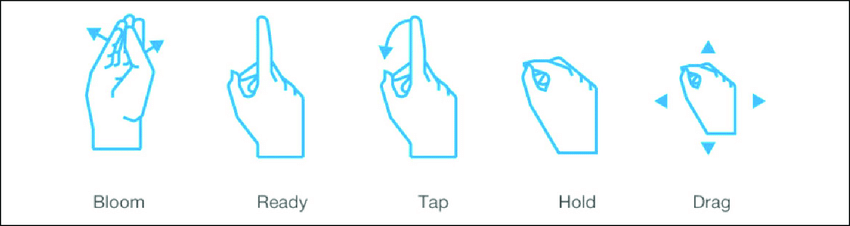
\includegraphics[width=0.7\linewidth]{images/hololensGestures.png}
	\caption{Handgesten, die die \textit{HoloLens} erkennt.}
	\label{img:hololensGestures}
	\source{Übernommen von: \cite{Tang18}}
\end{figure}
\FloatBarrier

\begin{figure}[!htb]
	\centering
	%https://next.reality.news/news/new-magic-leap-gesture-documentation-offers-insight-into-hands-will-make-its-digital-world-come-alive-0183614/
	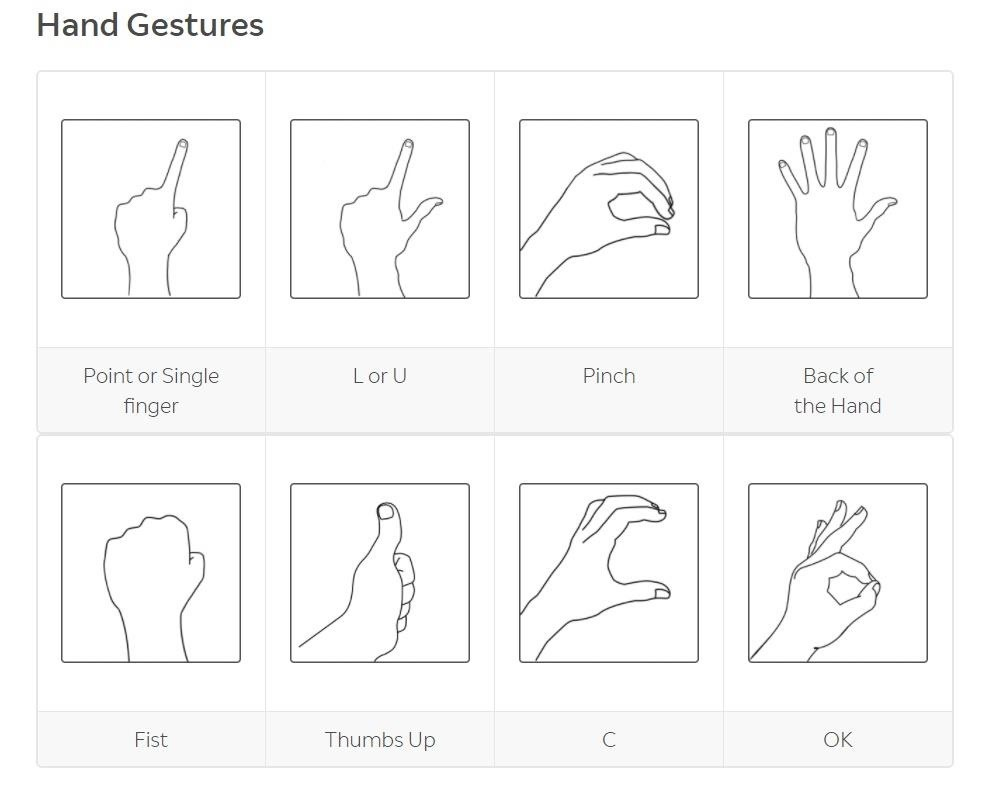
\includegraphics[width=0.7\linewidth]{images/magicleapGestures.jpg}
	\caption{Handgesten, die die \textit{Magic Leap} erkennt.}
	\label{img:magicGestures}
	\source{Übernommen von: https://next.reality.news/news/new-magic-leap-gesture-documentation-offers-insight-into-hands-will-make-its-digital-world-come-alive-0183614/}
\end{figure}
\FloatBarrier

\paragraph{Kopfposition und -drehung}

Bei einem HMD spielt die Position und Rotation des Kopfes eine zentrale Rolle. 
Derzeitige HMDs verwenden kein Eye-Tracking, um zu ermitteln worauf der Nutzer seinen Blick richtet, sodass der Nutzer, um sich beispielsweise umzusehen den ganzen Kopf drehen muss. Die Bewegung des Kopfes dient dem Nutzer also vor allem zur Navigation durch die erweiterte bzw. virtuelle Realität. 

Im Fall der \textit{HoloLens} bewegt der Nutzer dadurch nicht nur die virtuelle Kamera durch die 3D-Szene, sondern steuert auch einen Cursor, der sich in einem gewissen Abstand vor ihm im Zentrum seines Blickfeldes befindet. Ähnlich eines Maus-Cursors kann er damit mit virtuellen Elementen interagieren. Trifft der Cursor auf ein Objekt, z.B. einen Knopf kann der Nutzer dieses entsprechend der Funktionsweise einer Maus per \textit{Air-Tap} anklicken. 

\paragraph{Sprachsteuerung}

Sprachsteuerung stellt eine weitere elementare Nutzereingabe der \textit{HoloLens} dar. 
Die meisten Befehle, wie das Öffnen von Apps und die Navigation durch Menüs in der \textit{HoloLens} können durch Sprachsteuerung gegeben werden. 
Dies liegt wahrscheinlich an der begrenzten und teilweise umständlichen Steuerung durch Gesten. Da eine Sprachsteuerung von \textit{HoloLens}-Apps vorgesehen ist, können von Entwicklern mit wenig Aufwand eigene Sprachbefehle registriert werden.
Das \textit{Vive}-System wird primär durch entsprechende Controller gesteuert. Die Brille besitzt allerdings auch ein integriertes Mikrofon, durch das Sprachbefehle entgegen genommen werden können.

%\paragraph{HMD-Knöpfe}
%Schließlich besitzen in vielen Fällen auch die HMDs der Systeme Knöpfe oder Räder. Diese dienen allerdings meistens zur Konfiguration des Systems und Steuern z.B. die Lautstärke.
%Linsenabstand? Capture?

\subsection{\textit{Leap Motion}}

Die \textit{Leap Motion} von \cite{leapMotion} ist ein externes Gerät, dass die Hände des Nutzers verfolgt und die genauen Handbewegungen über ein Kabel an einen Computer übermittelt. 
Um die Informationen zu sammeln, ist die \textit{Leap Motion} mit drei Infrarotemittern und zwei Kameras ausgestattet (vgl. \cite{Weichert13}). Das Gerät wird über USB an einen Rechner angeschlossen und kann als unabhängiges Eingabemedium verwendet werden. Allerdings ist auch eine Verwendung in Kombination mit AR- oder VR-Systemen möglich. 
Die \textit{Leap Motion} schafft es die Handbewegungen des Nutzers nachzuempfinden, sodass die Hände in den digitalen Raum übertragen werden können. Hier kann nun eine Interaktion mit anderen digitalen Objekten stattfinden. Das Gerät erfasst dabei Bewegungen in einem Bereich von 150°x120° \cite{leapFOV}.
Wie in Kaptel \ref{konzept} erläutert wird, wird die die \textit{Leap Motion} mit einem HMD kombiniert, um dem Nutzer die Möglichkeit zu geben mARt mit seinen Händen zu steuern.








